\documentclass[10pt,twocolumn,letterpaper]{article}

\usepackage{epsfig}
\usepackage{graphicx}
\usepackage{amsmath}
\usepackage{amssymb}
\usepackage[breaklinks=true,bookmarks=false]{hyperref}
\usepackage{float}
\usepackage{caption}
\usepackage{enumitem}

\def\cvprPaperID{****} % Enter the CVPR Paper ID here
\def\httilde{\mbox{\tt\raisebox{-.5ex}{\symbol{126}}}}

\raggedright
\setcounter{page}{1}
\begin{document}

%%%%%%%%% TITLE
\title{Business Economic and Financial Data Project}

\author{
Flavio Kaci\\
{\tt\small 2124007}
\and
Antonio Mattesco\\
{\tt\small 2104368}
\and 
Alberto Calabrese\\
{\tt\small 2103405}
}

\date{}
\maketitle


\section{Introduction}
The culinary arts have always held a special place in the cultural and economic landscape of Italy, with each region offering its unique contributions to the nation’s gastronomic heritage. In Treviso, a city renowned for its historical charm and vibrant culinary traditions, one laboratory has distinguished itself through its artisanal approach to preparing delicacies for local gastronomy shops. Among its offerings, the signature dish—baccalà—has become a hallmark of excellence and a key driver of demand. This report aims to delve into the time series data surrounding this iconic product, shedding light on its production and consumption patterns while exploring predictive insights.

The analysis is rooted in data collected from the laboratory’s operations, focusing specifically on the production and supply metrics for baccalà. These metrics are critical not only for optimizing internal processes but also for ensuring consistent supply to meet the expectations of gastronomy shops and, by extension, the customers they serve. By leveraging advanced statistical techniques and predictive modeling, the goal is to identify trends, seasonality, and potential anomalies in the data, thereby enabling the laboratory to make informed decisions regarding inventory management and resource allocation.

A key objective of this report is to develop a robust short-term forecasting model. Accurate predictions are essential for maintaining the delicate balance between supply and demand, especially given the perishable nature of food products and the seasonal fluctuations that characterize the culinary industry. The predictive insights derived from this analysis will provide the laboratory with actionable intelligence, facilitating strategic planning and enhancing its capacity to respond proactively to market dynamics.

In addition to its operational benefits, this analysis seeks to underscore the broader implications of data-driven decision-making within the food industry. By adopting a methodical approach to time series analysis, the laboratory not only strengthens its competitive position but also contributes to the sustainability of local gastronomy. This aligns with a growing emphasis on efficiency and resilience within the supply chain, particularly in an era marked by evolving consumer preferences and increasing awareness of food waste.

Through this report, our aim is to combine the richness of tradition with the precision of modern analytics, providing a comprehensive understanding of the factors that influence the production and distribution of baccalà in Treviso. By examining historical data and projecting future trends, we seek to equip the laboratory with the tools it needs to continue thriving in a competitive and ever-changing market.

\section{Data}
\subsection{Data Gathering}
The data analyzed in this report were sourced from the archival records of the billing software utilized by the laboratory. This software has proven instrumental in compiling a comprehensive dataset on baccalà sales, spanning a period from January 2021 to December 2024. The dataset consists of 48 monthly observations, providing a robust foundation for time-series analysis.

Each observation in the dataset is structured into three columns:
\begin{itemize}
    \item Date: Represents the specific month and year of the recorded sale.
    \item Baccalà\_Mantecato: Indicates the quantity (in kg) of Baccalà Mantecato sold during the corresponding period.
    \item Baccalà\_Vicentina: Indicates the quantity (in kg) of Baccalà alla Vicentina sold during the corresponding period.
\end{itemize}


This dataset offers valuable information on the dynamics of baccalà production and consumption, allowing the identification of patterns and trends that can inform strategic decision making. By examining these variables over time, we aim to uncover the underlying factors influencing demand and develop predictive models to improve operational efficiency.

\subsection{Data Preprocessing}
To ensure the data was ready for analysis, several preprocessing steps were undertaken. Firstly, the "Date" column was converted into an appropriate date format, allowing for accurate temporal analysis. Additional features such as "Month" and "Year" were derived from the "Date" column to facilitate the identification of seasonal trends and interannual variations. A trend variable was also introduced to capture the temporal progression of the dataset.

Missing values were checked and confirmed to be absent, ensuring the dataset's integrity. Alongside the primary dataset, an external dataset containing information on salmon consumption in Italy was integrated. This dataset, sourced from \href{https://eumofa.eu/first-sale-weekly-data}{EUMOFA}, provided monthly observations on salmon sales, starting from January 2009. The inclusion of this dataset was motivated by its potential to serve as an explanatory variable in modeling baccalà sales.

The salmon dataset included three key variables:

Date: The month and year of salmon consumption, starting from November 2020. A two-month lag was applied to align with future forecasting scenarios.
\begin{itemize}
    \item kg\_std: The standardized quantity of salmon consumed (in kilograms), used to simplify comparative analysis.
    \item kg: The raw quantity of salmon consumed (in kilograms).
\end{itemize}

These data were aggregated and aligned with the baccalà dataset to ensure temporal consistency and compatibility. While other external variables, such as the NIC for fish products and production prices sourced from Istat, were initially considered, they were excluded due to their lack of statistical significance or mismatched temporal resolution.

The combined dataset now offers a comprehensive view of baccalà sales alongside relevant external factors, setting the stage for robust time series analysis and predictive modeling.

The resulting dataset, looks like:
\begin{table}[H]
\centering
\small
\begin{tabular}{|l|r|r|r|r|r|r|}
\hline
\textbf{Date} & \textbf{Mant.} & \textbf{Vic.} & \textbf{M.} & \textbf{Y.} & \textbf{Trend} & \textbf{Fish Cons} \\
\hline
2021-01-01 & 36.4 & 6.1 & 01 & 2021 & 1 & 0.8904992 \\
2021-02-01 & 36.4 & 5.4 & 02 & 2021 & 2 & 2.7444439 \\
2021-03-01 & 31.2 & 6.1 & 03 & 2021 & 3 & 0.6030702 \\
\hline
\end{tabular}
\caption{Resulting dataset}
\label{table:resulting_dataset}
\end{table}

\section{Explanatory Analysis}
The exploratory phase of the analysis begins with visualizing the time series data for Baccalà Mantecato and Baccalà Vicentina. This visualization provides a comparative view of the monthly sales trends for both products. Notably, the sales quantities of Baccalà Mantecato consistently exceed those of Baccalà Vicentina across all observed periods. Furthermore, Baccalà Mantecato demonstrates greater variability in sales, with a wider range of values, while Baccalà Vicentina exhibits a more stable pattern. Both products, however, show a pronounced increase in sales during the final months of each year, particularly in December.

\begin{figure}[H]
    \centering
    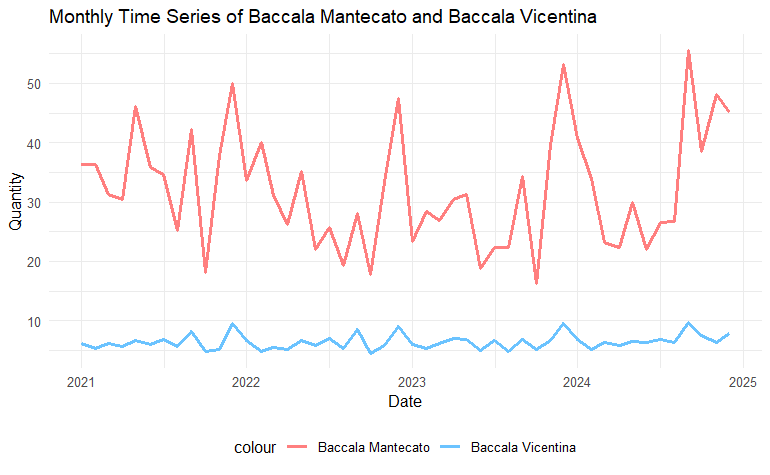
\includegraphics[width=0.5\textwidth]{PlotsBEFD/SS_MAN_VIC.png} 
    \caption{}
    \label{fig:esempio}
\end{figure}

To further explore yearly patterns, separate time series plots grouped by year were created for each product. These plots reveal consistent seasonal trends, with sales peaking in the latter months of the year, particularly in September and December. For Baccalà Mantecato, the data also suggest a shift over time: during the first year (2021), sales volumes in off-peak months were generally higher compared to subsequent years, while peak-month sales have increased in recent periods.
\begin{figure}[H]
    \centering
    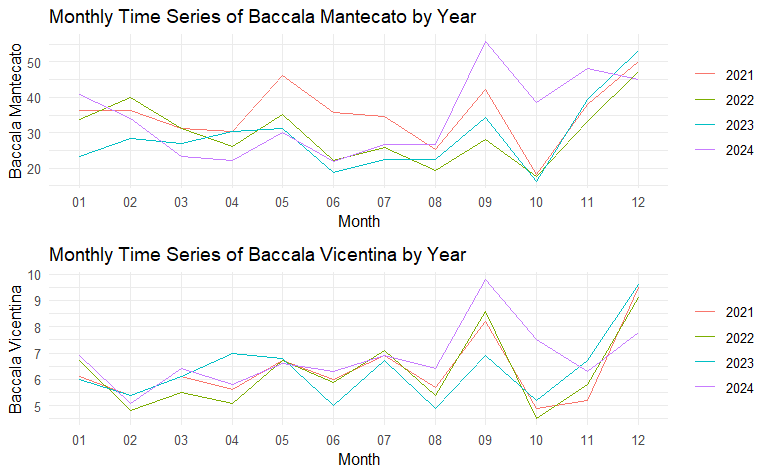
\includegraphics[width=0.5\textwidth]{PlotsBEFD/Month_SS_MAN_VIC.png} 
    \caption{}
    \label{fig:esempio}
\end{figure}

The autocorrelation functions (ACF) of the time series were analyzed to examine the presence of seasonality and lagged relationships. 
\begin{figure}[H]
    \centering
    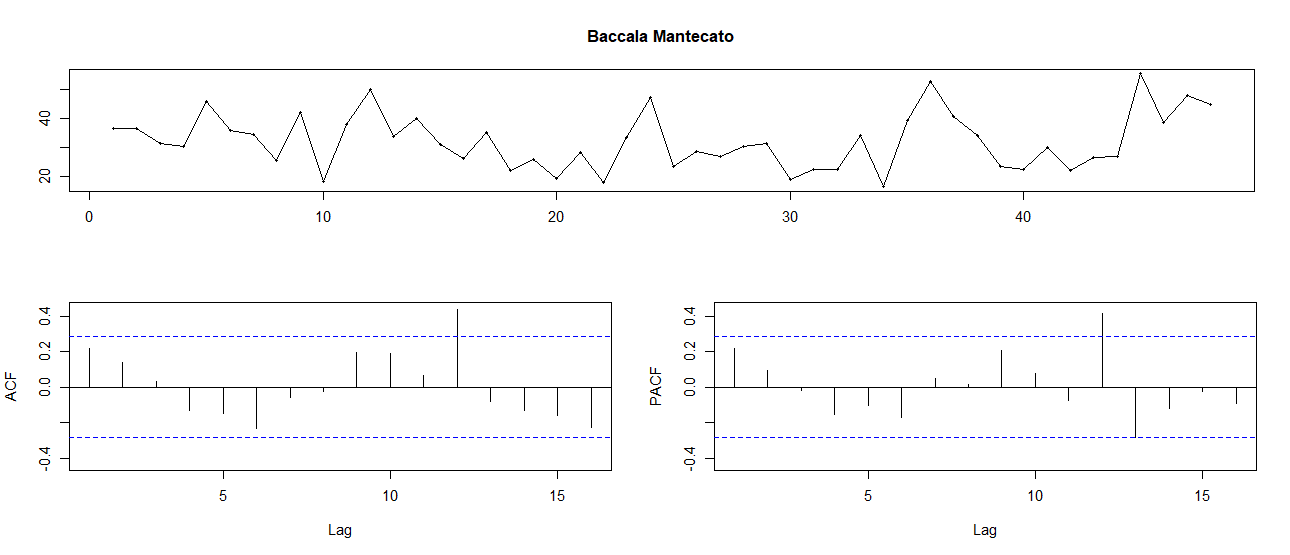
\includegraphics[width=0.5\textwidth]{PlotsBEFD/ACF_MAN.png} 
    \caption{}
    \label{fig:esempio}
\end{figure}
\begin{figure}[H]
    \centering
    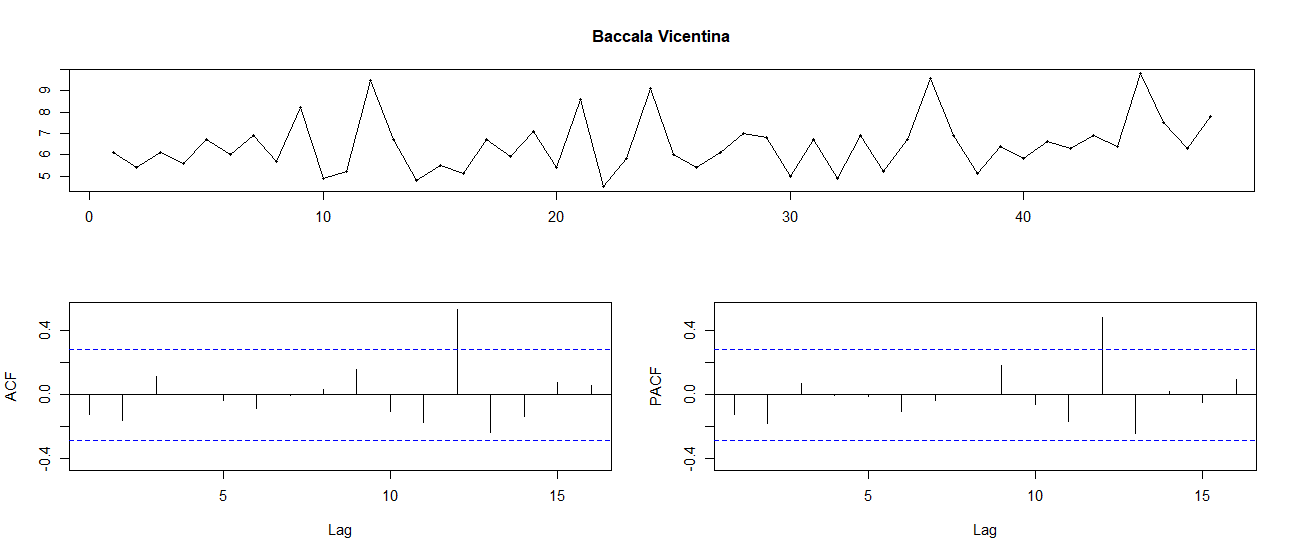
\includegraphics[width=0.5\textwidth]{PlotsBEFD/ACF_VIC.png} 
    \caption{}
    \label{fig:esempio}
\end{figure}
Most autocorrelations fall within the confidence bands, indicating an absence of significant correlation for most lags. However, the sinusoidal pattern observed within the bands suggests periodic fluctuations, with a notable peak at lag 12, supporting the hypothesis of annual seasonality. This periodic effect will be further evaluated by analyzing the residuals of future forecasting models to confirm or refute the presence of seasonality.

The insights gained from this exploratory analysis lay the groundwork for constructing robust predictive models that incorporate both seasonal and trend components. These models aim to enhance the laboratory's ability to forecast sales and optimize inventory management, ultimately contributing to its operational efficiency and market responsiveness.

\section{Train-Test Split}
To evaluate the predictive performance of forecasting models, the dataset was divided into training and testing subsets.

The training set includes observations from the initial 80\% of the time periods, while the test set consists of the final 20\%. By design, this approach preserves the temporal structure of the data, preventing data leakage and ensuring that predictions are based solely on prior information.

For visualization purposes, the split was applied to both Baccalà Mantecato and Baccalà Vicentina. Two distinct plots illustrate the separation between training and testing data for each product. These plots reveal the temporal trends in sales, highlighting the segments used for model training and evaluation.

\begin{figure}[H]
    \centering
    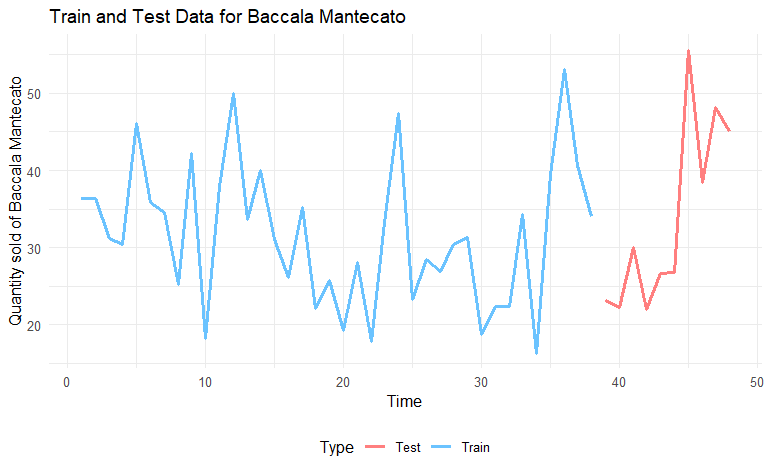
\includegraphics[width=0.5\textwidth]{PlotsBEFD/TRAIN_TEST_MAN.png} 
    \caption{}
    \label{fig:esempio}
\end{figure}
Baccalà Mantecato: The training data (in blue) exhibits the characteristic variability and seasonal trends observed in the explanatory analysis. The testing data (in red) includes more recent observations, capturing the peak sales periods in September and December.
\begin{figure}[H]
    \centering
    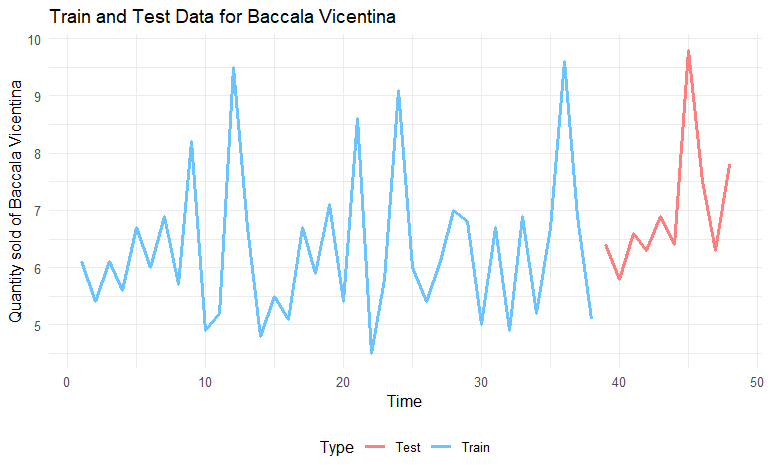
\includegraphics[width=0.5\textwidth]{PlotsBEFD/TRAIN_TEST_VIC.png} 
    \caption{}
    \label{fig:esempio}
\end{figure}
Baccalà Vicentina: Similarly, the training data reflects the stable yet seasonal nature of sales, while the testing data emphasizes the end-of-year peaks.

Notably, in 2024, the peak sales for Baccalà occurred in September rather than December, deviating from historical patterns. This anomaly may present challenges for forecasting models, as it represents a shift in seasonal behavior for both the variants.

By implementing this train-test split, the analysis sets the stage for rigorous model development and validation. 
%%The observed deviations in 2024 underscore the importance of incorporating mechanisms to handle potential anomalies and shifts in seasonal trends, ensuring robust and reliable predictions. LA RIMUOVERI PERCHE NOI QUESTA CHALLENGE NON LA AFFRONTIAMO, NE SIAMO SOLO PENALIZZATI

\section{Modelling}
\subsection{Linear Regression Models}
The modeling phase began with the development of linear regression models for both Baccalà Mantecato and Baccalà Vicentina. Each variant required a distinct approach due to their different underlying patterns and relationships with predictor variables.

\subsubsection{Model for Baccalà Mantecato}
For Baccalà Mantecato, the initial model incorporated three key predictors: a trend variable, monthly seasonality indicators, and fish consumption data. The model demonstrated strong explanatory power, with an R-squared value of 0.9178, indicating that approximately 91.78\% of the variability in Baccalà Mantecato sales could be explained by these predictors.
Analysis of the coefficients revealed several important relationships:

The trend variable showed a positive coefficient of 0.18, suggesting that, ceteris paribus, Baccalà Mantecato sales increase by 0.18 units per time period.
Fish consumption demonstrated a strong positive relationship with a coefficient of 7.79, indicating that for each unit increase in fish consumption, Baccalà Mantecato sales rise by approximately 7.79 kg. For example, if fish consumption in Italy increases by one unit in October 2021, the quantity sold in December 2021 would increase by 7.79 kg, assuming all other variables remain constant
The monthly indicators captured significant seasonal effects, with December showing a substantial positive impact and months like February and October displaying negative coefficients relative to the January baseline

Model selection was performed by systematically removing variables and comparing performance metrics (AIC and adjusted R²) across different specifications:
\begin{itemize}[noitemsep, topsep=0pt]
    \item Model with trend and fish consumption only
    \item Model with trend and monthly seasonality only
    \item Model with monthly seasonality and fish consumption only
    \item Full model with all predictors
\end{itemize}
The comparative analysis confirmed that the full model, incorporating all predictors, provided the best fit according to both AIC and adjusted R² criteria.
\begin{figure}[H]
    \centering
    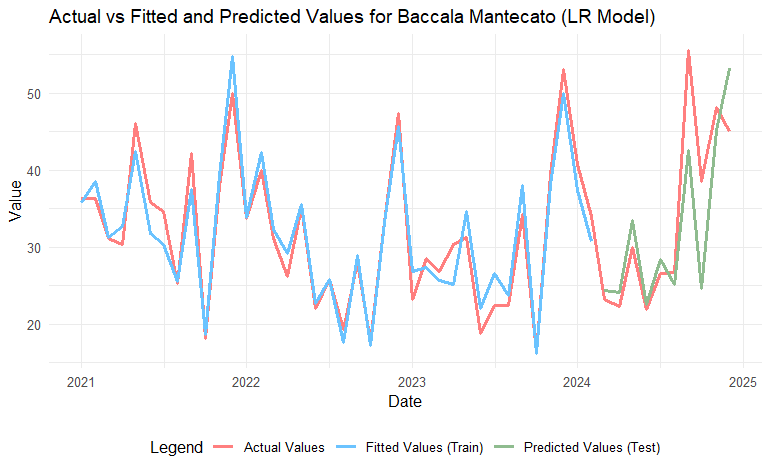
\includegraphics[width=0.5\textwidth]{PlotsBEFD/PRED_LR_MAN.png} 
    \caption{}
    \label{fig:esempio}
\end{figure}
Residual analysis revealed no concerning patterns, with residuals appearing randomly scattered, suggesting that the model's assumptions of linearity, constant variance, and independence were reasonably satisfied. The Durbin-Watson test for autocorrelation yielded a p-value below 0.05, supporting the null hypothesis that the residuals' autocorrelation is zero.
\begin{figure}[H]
    \centering
    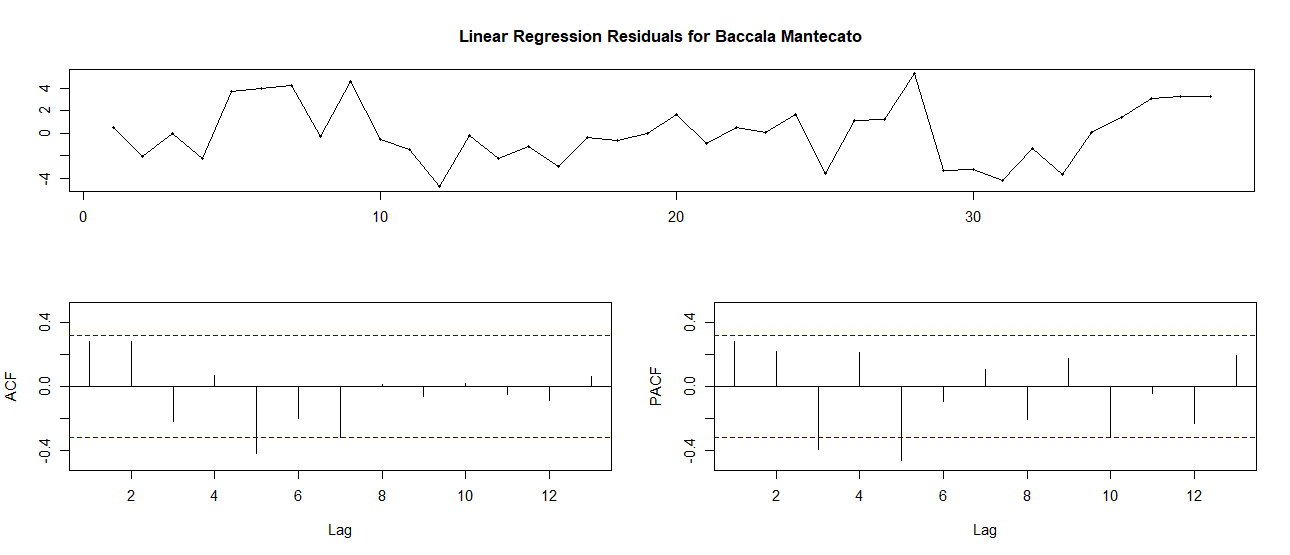
\includegraphics[width=0.5\textwidth]{PlotsBEFD/RES_LR_MAN.png} 
    \caption{}
    \label{fig:esempio}
\end{figure}

\subsubsection{Model for Baccalà Vicentina}
The modeling approach for Baccalà Vicentina followed a similar initial framework but led to different conclusions. The initial full model included the same three predictors: trend, monthly seasonality, and fish consumption. However, the analysis revealed that fish consumption did not significantly contribute to the model's performance.
Through iterative model refinement:

Fish consumption was removed, leading to an improvement in adjusted R² from 0.8261 to 0.8305
The trend variable was subsequently eliminated due to its high p-value
The final model retained only monthly seasonality indicators
\begin{figure}[H]
    \centering
    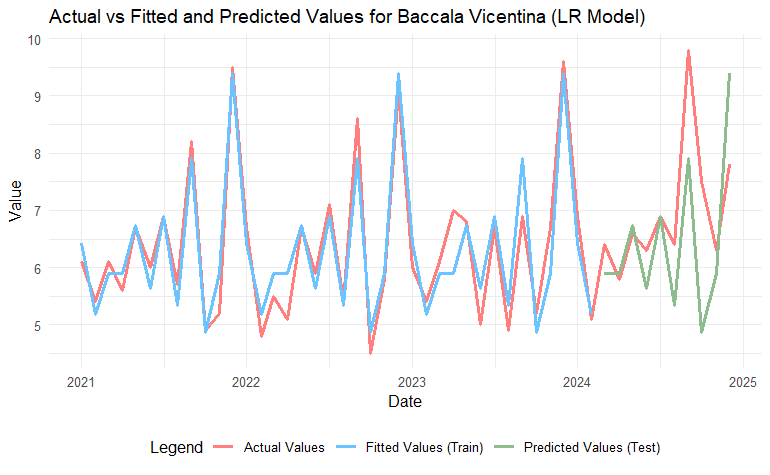
\includegraphics[width=0.5\textwidth]{PlotsBEFD/PRED_LR_VIC.png} 
    \caption{}
    \label{fig:esempio}
\end{figure}
The simplified model demonstrated strong statistical significance with an F-statistic of 18.21 (p-value: 1.684e-09). This suggests that variations in Baccalà Vicentina sales are primarily driven by seasonal effects, without significant influence from trend or fish consumption patterns.
Comparison of model performance metrics confirmed the superiority of the seasonality-only model over the full specification, with improved AIC and adjusted R² values. 
\newline
The analysis of the historical sales data for baccalà vicentina in kilograms reveals notable seasonal effects. December shows a significant positive impact on sales (+2.975), likely driven by higher demand during the holiday season. In contrast, October (-1.558) and February (-1.250) exhibit substantial declines compared to January. Additionally, August records a notable decrease (-1.092), potentially reflecting lower summer demand. These results highlight clear seasonal patterns in sales trends.
\newline
Residual analysis showed a problematic scatter, indicating problematic model fit. 
\begin{figure}[H]
    \centering
    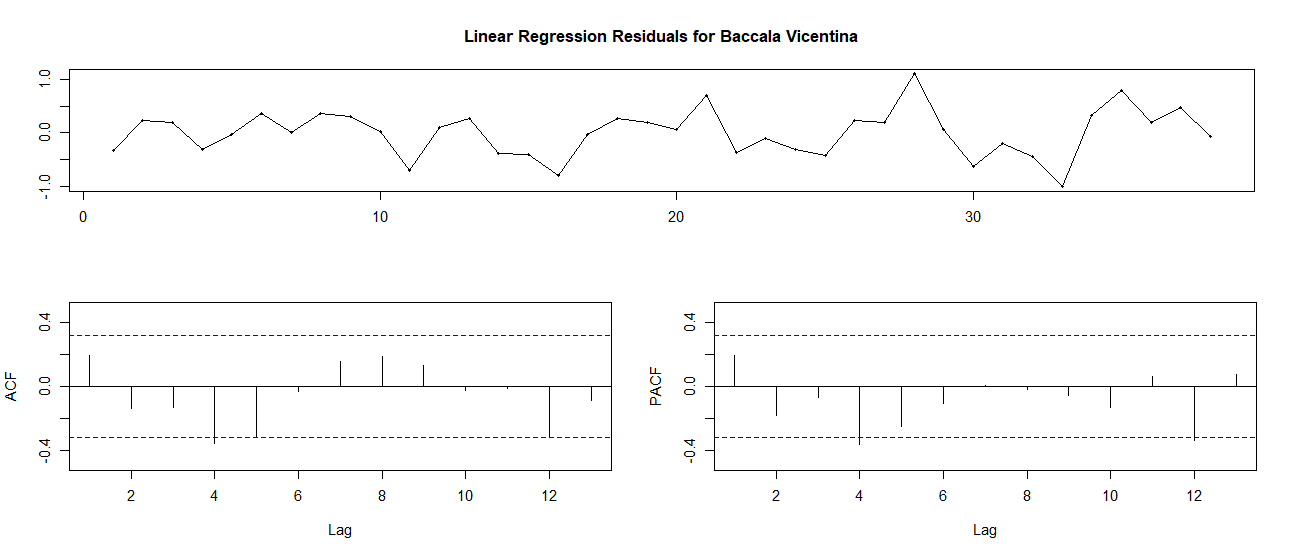
\includegraphics[width=0.5\textwidth]{PlotsBEFD/RES_LR_VIC.png} 
    \caption{}
    \label{fig:esempio}
\end{figure}
This idea is confirmed by the Durbin-Watson test, which suggested the presence of some autocorrelation in the residuals, as indicated by a p-value (0.18) exceeding the 0.05 significance level.
The distinct modeling outcomes for the two variants highlight the importance of tailored approaches in time series analysis, as similar products may exhibit different underlying patterns and relationships with predictor variables.

\subsection{SARIMA Models}
Following the linear regression analysis, we explored various time series models for both variants of baccalà. Initial attempts with ARMA and ARIMA models showed poor performance due to the pronounced seasonal patterns in the data. This led us to focus on Seasonal Autoregressive Integrated Moving Average (SARIMA) models, which explicitly account for seasonality in the time series.

\subsubsection{Model for Baccalà Mantecato}
Initial analysis of the Baccalà Mantecato time series confirmed the presence of both trend and seasonal components identified in the regression analysis. After transforming the data into a time series object, we examined the autocorrelation (ACF) and partial autocorrelation (PACF) functions of the first-differenced series. 

\begin{figure}[H]
    \centering
    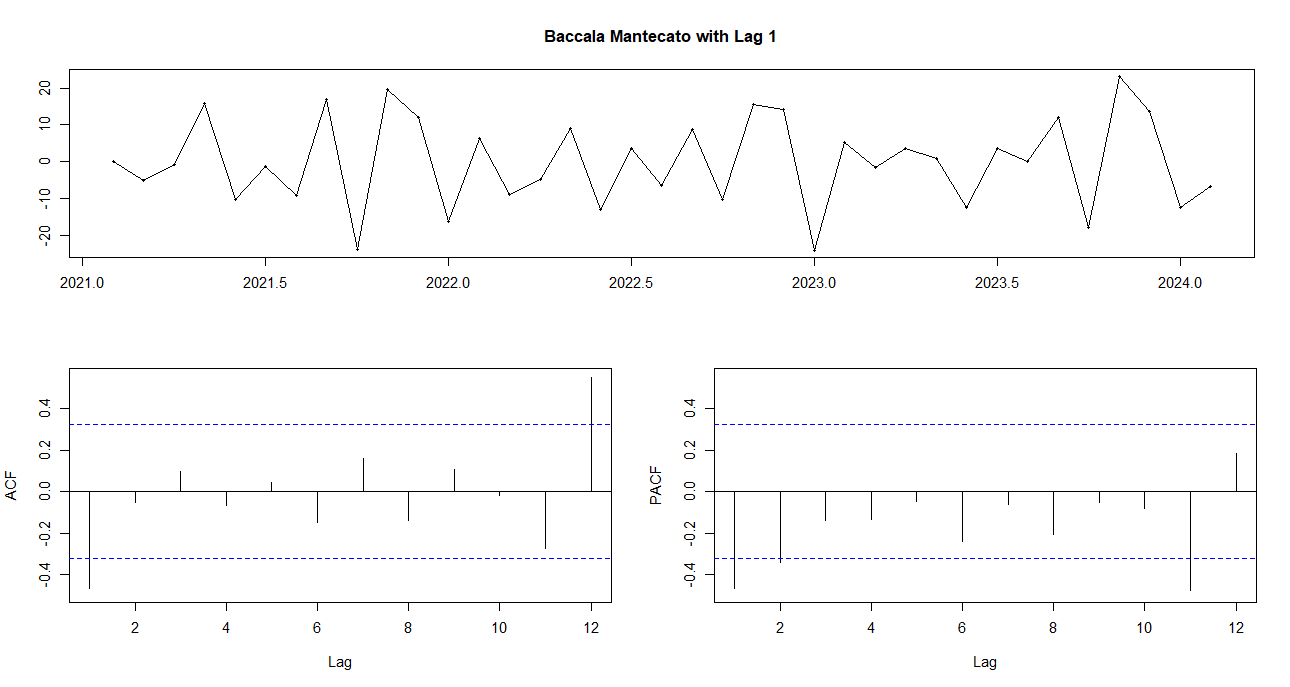
\includegraphics[width=0.5\textwidth]{PlotsBEFD/ACF_MAN_LAG1.png} 
    \caption{}
    \label{fig:esempio}
\end{figure}

Both ACF and PACF plots revealed a distinctive sinusoidal pattern, with values generally within the confidence bands except for a significant spike at lag 12, strongly suggesting annual seasonality in the data.
To address these patterns, three SARIMA models were evaluated:
\begin{itemize}[noitemsep, topsep=0pt]
    \item \textbf{SARIMA(1,1,0)(0,1,0)[12]}: Includes non-seasonal differencing (\(d=1\)), one autoregressive term, and seasonal differencing.
    \item \textbf{SARIMA(0,1,1)(0,1,0)[12]}: Incorporates a moving average term instead of an autoregressive term.
    \item \textbf{SARIMA(0,1,0)(0,1,0)[12]}: Uses only differencing components.
\end{itemize}

While the SARIMA(0,1,1)(0,1,0)[12] model showed the lowest AIC value, suggesting better in-sample fit, evaluation on the test set revealed that the simpler SARIMA(0,1,0)(0,1,0)[12] model achieved superior out-of-sample performance with lower Mean Squared Error (MSE). This finding highlights the importance of model parsimony and the potential risks of overfitting.
Analysis of the residuals for the selected model showed some patterns that suggest the fit isn't perfect.
\begin{figure}[H]
    \centering
    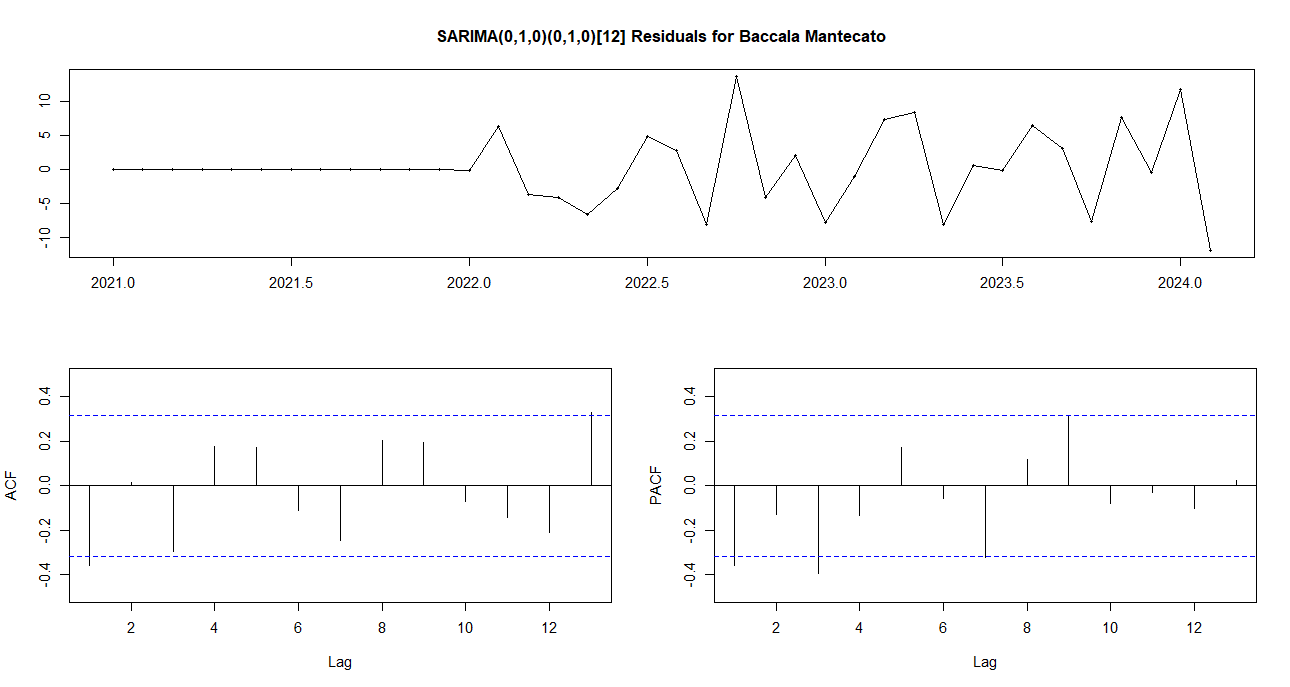
\includegraphics[width=0.5\textwidth]{PlotsBEFD/RES_ACF_SARIMA_MAN.png} 
    \caption{}
    \label{fig:esempio}
\end{figure}


However, given its superior test set performance, this model was retained as the final specification for Baccalà Mantecato.

\subsubsection{Model for Baccalà Vicentina}
For Baccalà Vicentina, the time series analysis revealed strong seasonal patterns, with the ACF and PACF functions showing significant spikes at lag 12, confirming the annual seasonality identified in the regression analysis. 
\begin{figure}[H]
    \centering
    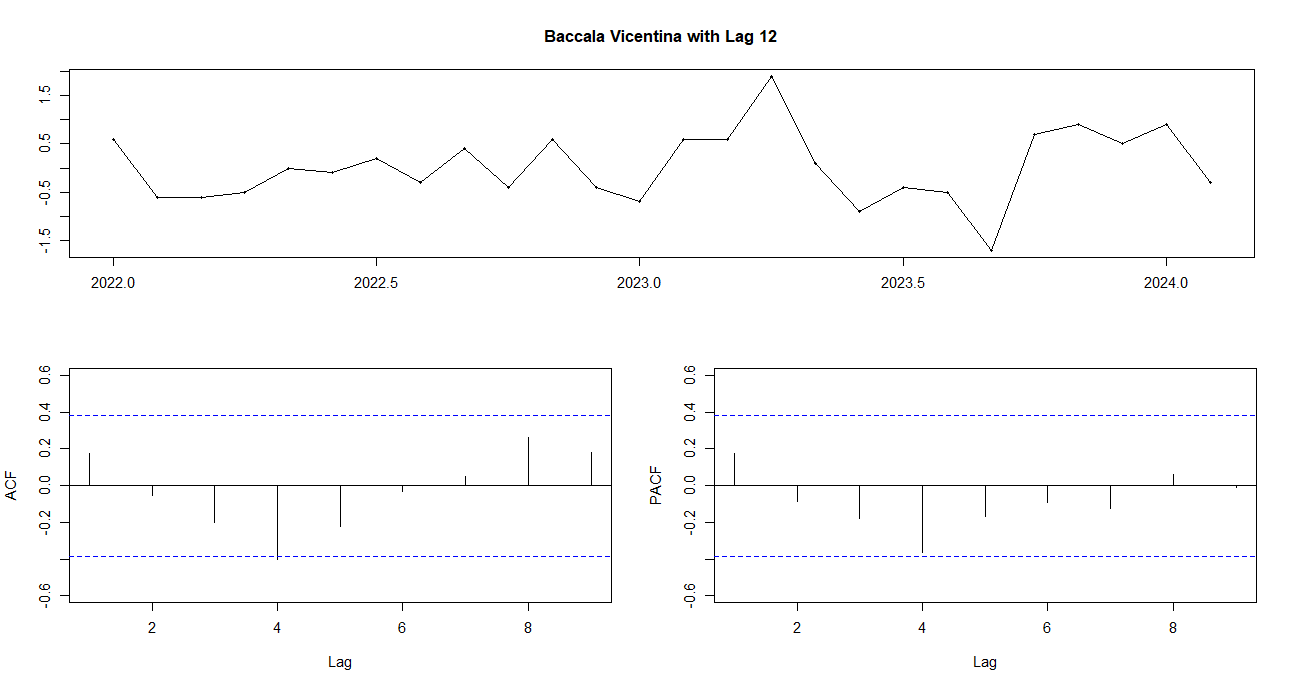
\includegraphics[width=0.5\textwidth]{PlotsBEFD/ACF_VIC_LAG12.png} 
    \caption{}
    \label{fig:esempio}
\end{figure}
Unlike Baccalà Mantecato, the series showed less evidence of trend components.
After examining various specifications, a SARIMA(0,0,0)(0,1,0)[12] model was selected.
While models with higher orders of seasonal differencing (D=2) produced lower AIC values, they led to higher MSE on the test set, indicating overfitting. The chosen model represents a balance between complexity and predictive accuracy.
\begin{figure}[H]
    \centering
    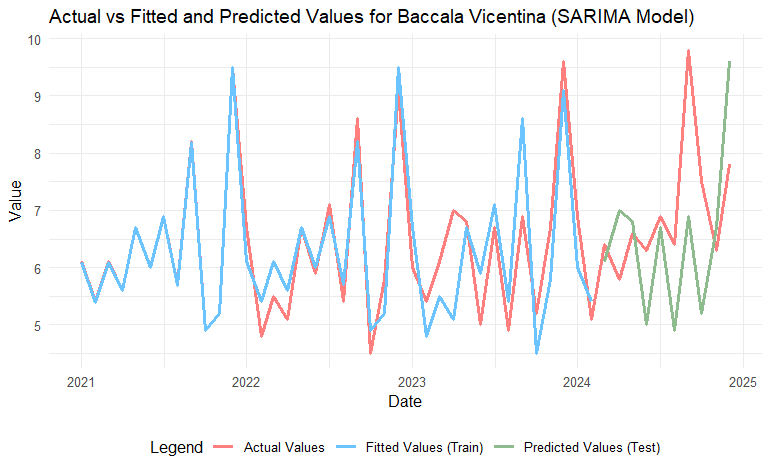
\includegraphics[width=0.5\textwidth]{PlotsBEFD/PRED_SARIMA_VIC.png} 
    \caption{}
    \label{fig:esempio}
\end{figure}
The residual analysis of the final model showed some remaining patterns, suggesting that while the model captures the main features of the series, there might be additional structure in the data. However, attempts to incorporate additional ARIMA components did not yield improved performance, supporting the retention of the simpler specification.



These SARIMA models complement the linear regression analysis by explicitly modeling the time series structure of the data, particularly the seasonal patterns that are crucial for both variants of baccalà. The different specifications required for each variant further emphasize the distinct temporal dynamics of these products, despite their related nature.

\subsection{SARIMAX Models}
To extend our previous analysis with SARIMA models, we included fish consumption as an external regressor (xreg) to assess whether it could enhance the predictive performance of the models. The rationale behind this choice is rooted in exploring potential relationships between fish consumption patterns and the demand for the specific products analyzed. Below, we describe the steps and results obtained for each product category.

\subsubsection{Baccalà Mantecato}

We tested three SARIMAX models using different parameter configurations, maintaining consistency with the previously defined SARIMA structures. Each model incorporated fish consumption data as an external regressor:
\begin{itemize}
    \item SARIMAX(1,1,0)(0,1,0)[12]
    \item SARIMAX(0,1,1)(0,1,0)[12]
    \item SARIMAX(0,1,0)(0,1,0)[12]
\end{itemize}

The comparison between the SARIMA and SARIMAX models was performed using AIC values as the primary metric. Notably, all SARIMAX models exhibited improved AIC scores compared to their SARIMA counterparts. However, recognizing the limitations of relying solely on AIC, we also evaluated the models using Mean Squared Error (MSE) on the test set predictions.

The MSE analysis revealed a significant improvement for all three SARIMAX models, with reductions of approximately 50\% compared to the SARIMA models. Considering both AIC and MSE, we selected the SARIMAX(0,1,0)(0,1,0)[12] model as the most suitable for forecasting Baccalà Mantecato.

To visualize the performance, we plot the actual versus predicted values for both SARIMA and SARIMAX on the test set. 
\begin{figure}[H]
    \centering
    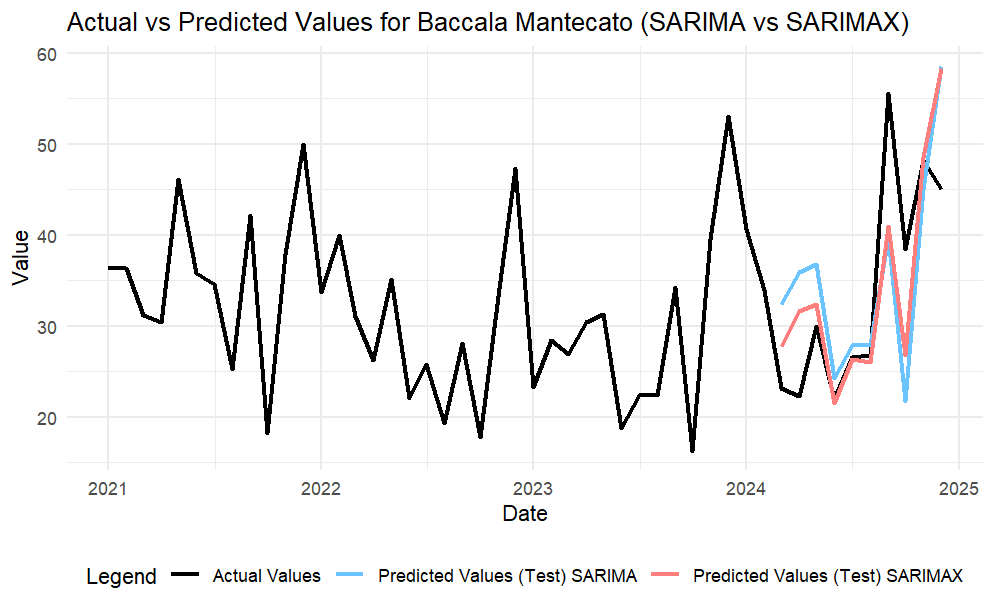
\includegraphics[width=0.5\textwidth]{PlotsBEFD/M_COMPARE_SARIMAX_SARIMA_TEST_PRED.png} 
    \caption{}
    \label{fig:esempio}
\end{figure}

The plot highlights the substantial improvement achieved with SARIMAX, confirming the utility of including fish consumption as an external regressor in this context.

Despite these positive results, the residual analysis of the selected SARIMAX model indicates some remaining autocorrelation, suggesting a potential need for an autoregressive component. 
\begin{figure}[H]
    \centering
    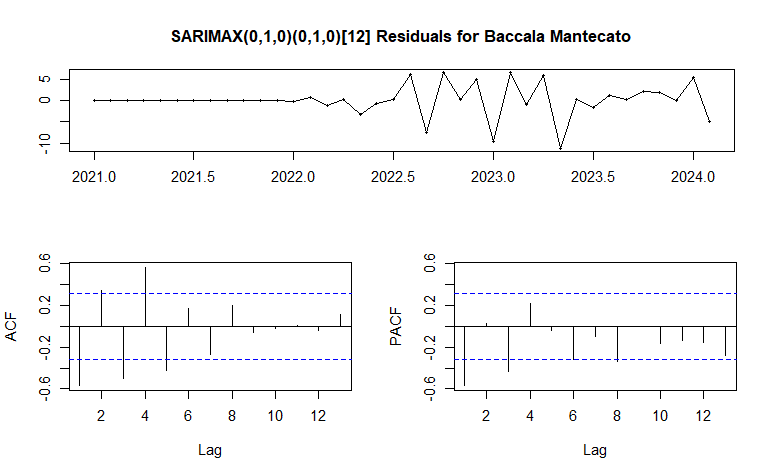
\includegraphics[width=0.5\textwidth]{PlotsBEFD/ACF_SARIMAX_M.png} 
    \caption{}
    \label{fig:esempio}
\end{figure}
However, introducing this component results in overfitting and worse test set performance, leading us to accept the slight loss of information in favor of generalization.

\subsubsection{Baccalà Vicentina}

For Baccalà Vicentina, we applied a similar approach, comparing the previously selected SARIMA(0,1,1)(0,1,0)[12] model with its SARIMAX counterpart, which included fish consumption as an external regressor:

SARIMAX(0,1,1)(0,1,0)[12]

The AIC and MSE evaluations for this product category yielded surprising results. Unlike Baccalà Mantecato, the SARIMA model consistently outperformed the SARIMAX model across both metrics. This discrepancy suggests that the inclusion of fish consumption data did not enhance the model’s predictive capabilities for Baccalà Vicentina.
\begin{figure}[H]
    \centering
    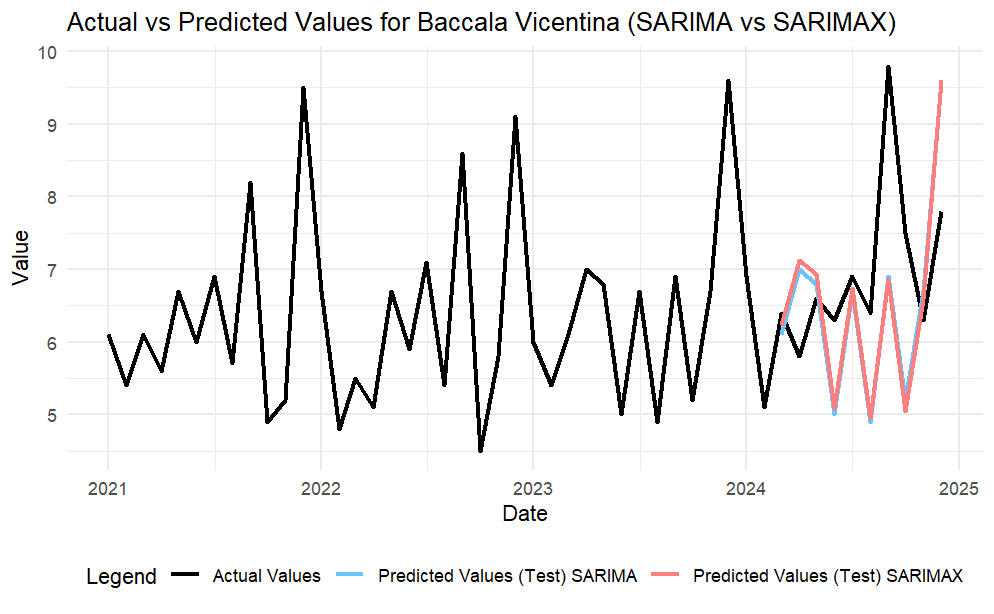
\includegraphics[width=0.5\textwidth]{PlotsBEFD/V_COMPARE_SARIMAX_SARIMA_TEST_PRED.png} 
    \caption{}
    \label{fig:esempio}
\end{figure}
A closer examination of the prediction plots revealed that both models produced similar trends. However, the SARIMAX model appeared to overestimate quantities during the test period, coinciding with a recurring December peak absent in the test set. This overestimation likely contributed to the inferior performance of the SARIMAX model, as indicated by the higher AIC and MSE values.

Consequently, we decided to retain the original SARIMA model for Baccalà Vicentina, as the inclusion of fish consumption did not provide a tangible benefit and introduced a risk of overfitting.


The comparative analysis between SARIMA and SARIMAX models demonstrates the importance of context-specific considerations when incorporating external regressors. While fish consumption significantly improved the predictive accuracy for Baccalà Mantecato, it had the opposite effect for Baccalà Vicentina. These findings highlight the nuanced relationship between external factors and product demand, emphasizing the need for tailored modeling approaches in time series forecasting.

\subsection{GAM models}
\subsubsection{Baccalà Mantecato}
In this analysis, we aimed to explore the potential benefits of non-linear models, using Generalized Additive Models (GAM), and compared them to the previously selected Multiple Linear Regression model. Initially, we fitted the MLR model and then examined the linear effects through GAM to assess the possibility of improving the fit with non-linear relationships.

Upon visual inspection of the plots, it was evident that the relationship between the predictors and the response variable was clearly linear. 
\begin{figure}[H]
    \centering
    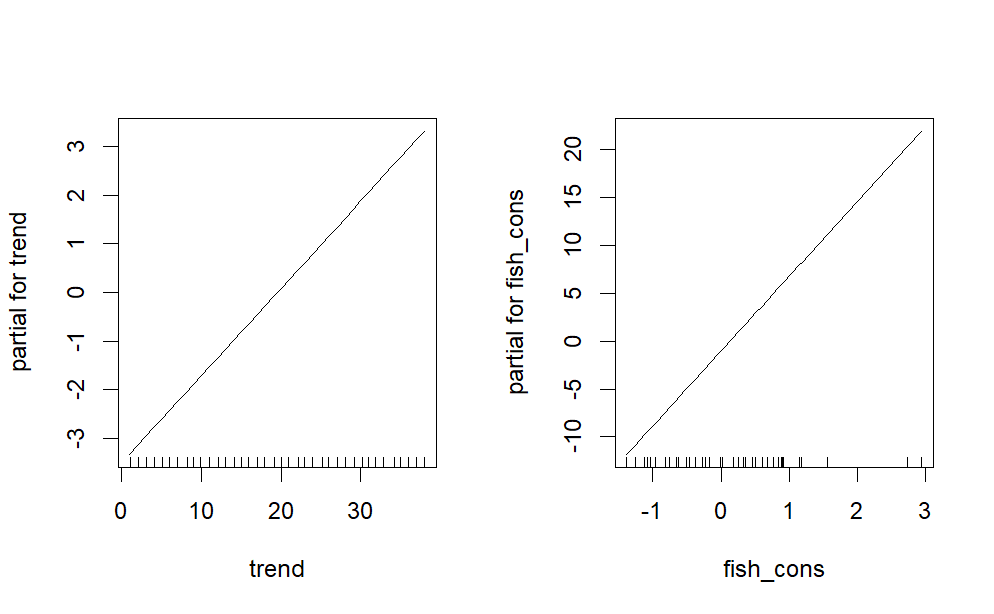
\includegraphics[width=0.5\textwidth]{PlotsBEFD/GAM_M_LINEARITY.png} 
    \caption{}
    \label{fig:esempio}
\end{figure}
This observation was further supported by the statistical results from the 'Anova for Nonparametric Effects', which showed that the nonparametric F-values for the smoothing terms s(trend) and s(fish\_cons) were not statistically significant, with p-values of 0.19 and 0.08, respectively.
These results strongly indicate that these variables do not exhibit non-linear relationships with the response variable as initially hypothesized.

Therefore, for parsimony, interpretability, and simplicity reasons, we concluded that the GAM model was unnecessary and opted to exclude it in favour of the multiple linear regression model. This model not only aligns better with the data but also provides more meaningful and statistically sound results, consistent with the initial assumption of linearity.

\subsubsection{Baccalà Vicentina}
For Baccalà Vicentina, we followed a similar approach by fitting a GAM model to check for non-linear relationships. However, as with Baccalà Mantecato, the plots clearly demonstrated that the relationship between the explanatory variables and the response variable remained linear. This again suggested that the non-linear modeling approach was not needed.

Moreover, in the section dedicated to linear regression, we had already determined that the best model for Baccalà Vicentina was the reduced model, where only the Month variable was included as a predictor. Given that this model was the most effective, we decided to retain it.

In conclusion, both analyses—Baccalà Mantecato and Baccalà Vicentina—strongly suggest that non-linear models, such as GAMs, are not necessary in this case. The evidence indicates that linear models are sufficient for capturing the relationships in the data, and choosing them over GAMs offers a more parsimonious, interpretable, and statistically sound solution.

\subsection{Prophet model}
For the Prophet model, two distinct models are created for each dish: one with logistic growth and one with linear growth. The choice of model depends on the nature of the data, but both models include yearly seasonality, which is crucial to capturing the seasonal cycles typical of food sales, especially for traditional dishes like Baccalà. The parameter n.changepoints=5, that is selected after several tries, trying do avoid overfitting but also to reach a good fit, specifies the number of points in time where the series can experience structural changes. Finally a multiplicative seasonality is selected for both dishes.
\subsubsection{Baccalà Mantecato}
We adapted the model for the Mantecato sales data, and the residuals revealed some issues, particularly highlighted by both the PACF and ACF plots, especially with the spike at lag 12. Despite this, attempts to improve the model by increasing the number of change points or experimenting with different specifications led to a deterioration in performance on the test set.

We also tried to incorporate a model estimated on the residuals using the `auto.arima` function, but this did not improve the model's performance. Given these results, we decided to retain the original Prophet model for its simplicity, as further adjustments did not yield better predictive accuracy.

\begin{figure}[H]
    \centering
    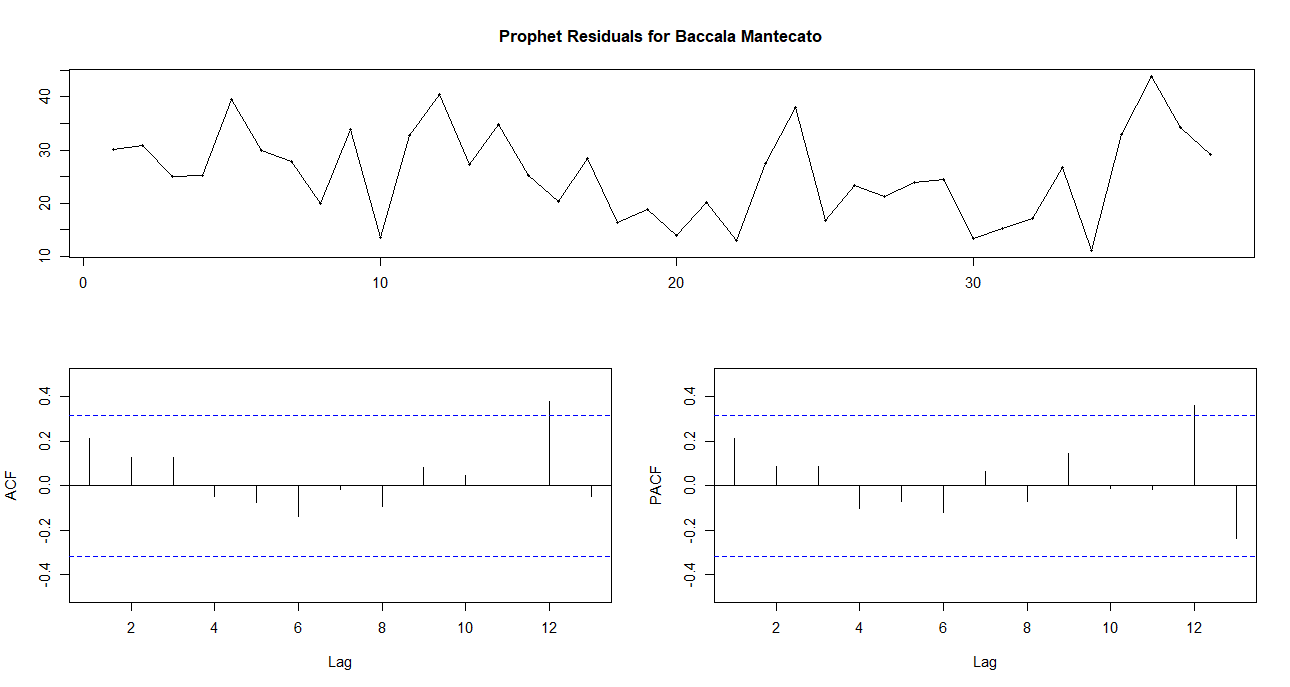
\includegraphics[width=0.5\textwidth]{PlotsBEFD/RES_PROPHET_MAN.png} 
    \caption{}
    \label{fig:esempio}
\end{figure}

Finally, in the graph below, we show the predicted values versus the actual values. From the graph, we can observe a good fit to the training data, but the same issues as with the other models are evident on the test set.
\begin{figure}[H]
    \centering
    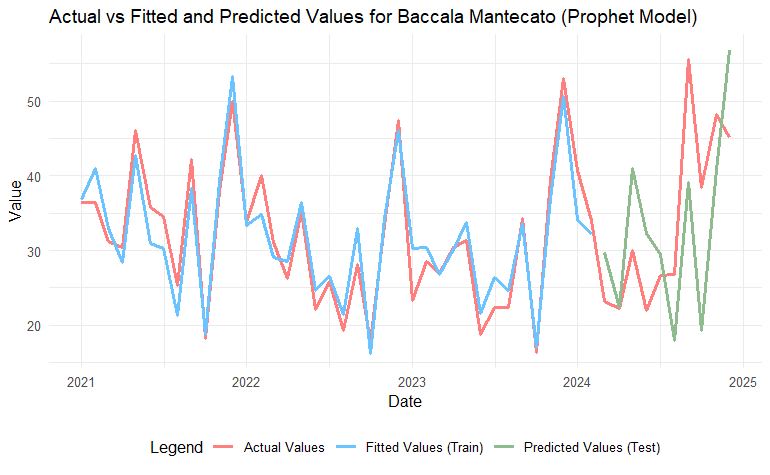
\includegraphics[width=0.5\textwidth]{PlotsBEFD/PRED_PROPHET_MAN.png} 
    \caption{}
    \label{fig:esempio}
\end{figure}

\subsubsection{Baccalà Vicentina}
The same behavior is observed for Baccalà alla Vicentina, where the residuals show a spike at lag 12. However, we do not want to dwell too much on repeating the same observations, so for completeness, we are including the graph of the actual values versus the predicted values.
\begin{figure}[H]
    \centering
    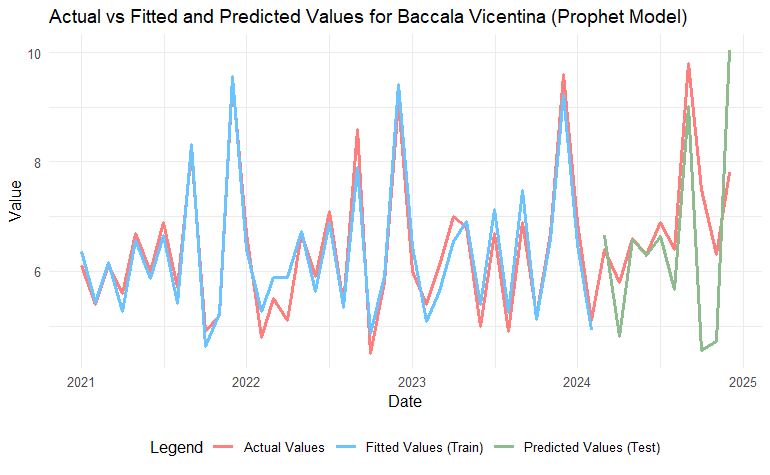
\includegraphics[width=0.5\textwidth]{PlotsBEFD/PRED_PROPHET_VIC.png} 
    \caption{}
    \label{fig:esempio}
\end{figure}

\subsection{Exponential smoothing Models}
After exploring other approaches, we decided to test Exponential Smoothing (ES) models to analyze and forecast the time series data for Baccalà Mantecato and Baccalà Vicentina. These models are particularly valued for their simplicity and their ability to assign exponentially decreasing weights to past observations, emphasizing the most recent data. They also offer flexibility in handling trend and seasonality, making them ideal for time series with recurring patterns.
For both datasets, we began by testing the classic ETS model (Error, Trend, Seasonality), an approach that automatically selects the optimal configuration based on the data.

\subsubsection{Baccalà Mantecato}
For the Baccalà Mantecato series, the ETS model effectively captured the key dynamics of the data, providing a strong baseline for further analysis. The model demonstrated its ability to adapt to the trends and seasonality present in the series, which were confirmed by both visual and statistical evaluations.
\begin{figure}[H]
    \centering
    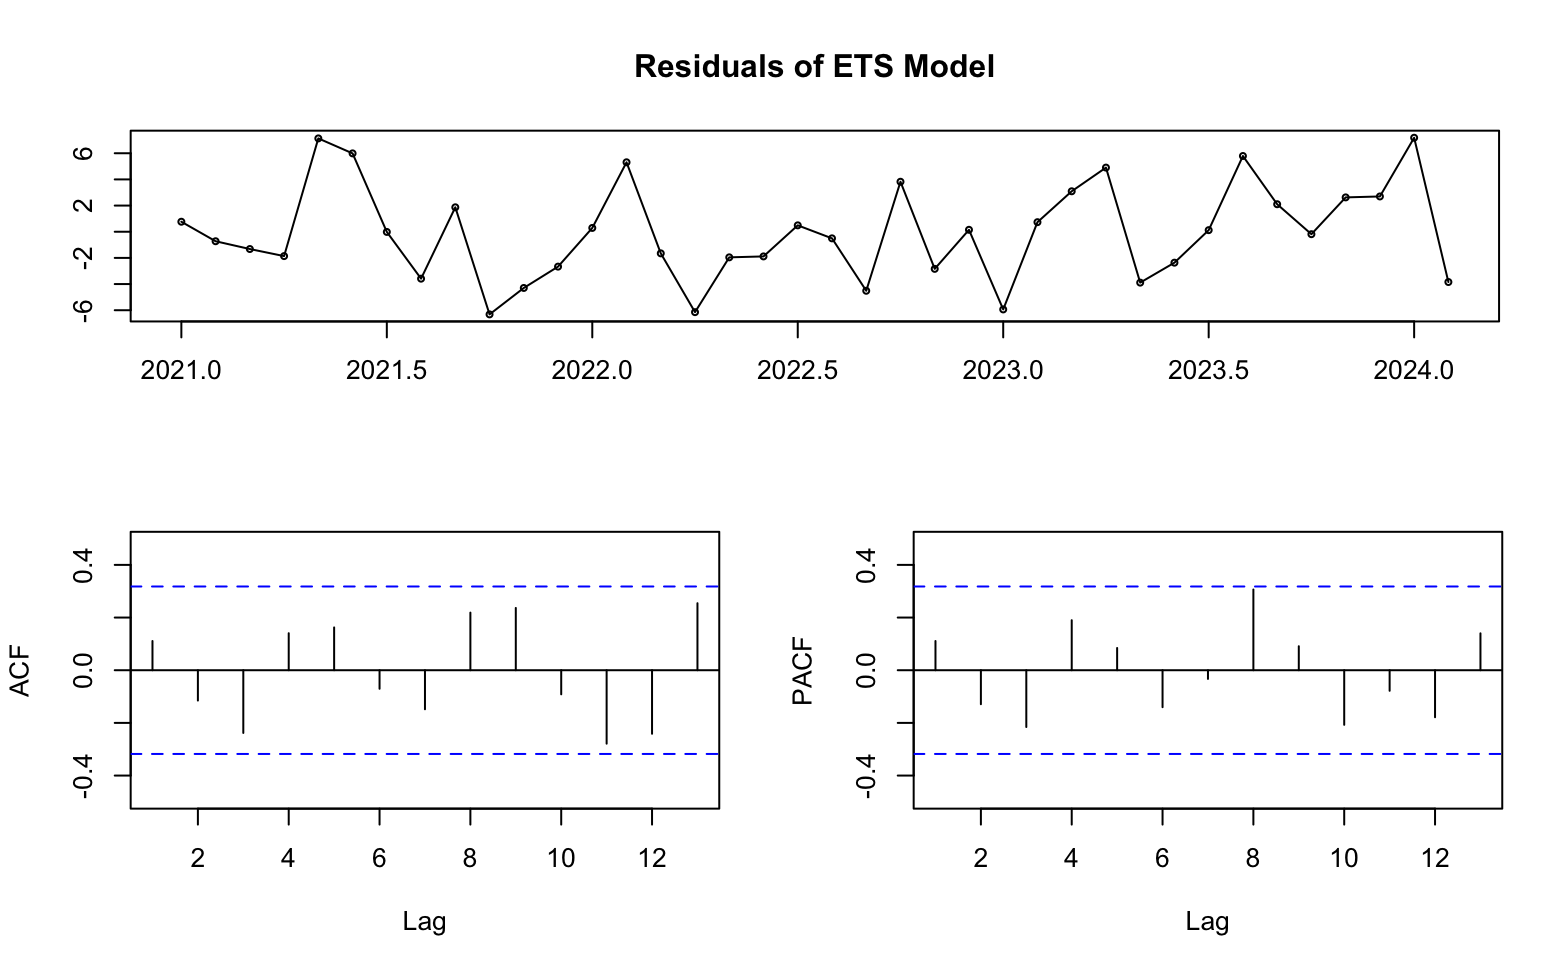
\includegraphics[width=0.5\textwidth]{PlotsBEFD/Residuals_ETS_M.png} 
    \caption{}
    \label{fig:esempio}
\end{figure}
Residual analysis revealed that the residuals were randomly distributed around zero, with no significant patterns or autocorrelation. This indicates that the model successfully accounted for the underlying trends and seasonality, leaving minimal systematic errors. Such behavior is a positive indication of the effectiveness of the ETS model for this time series.
\begin{figure}[H]
    \centering
    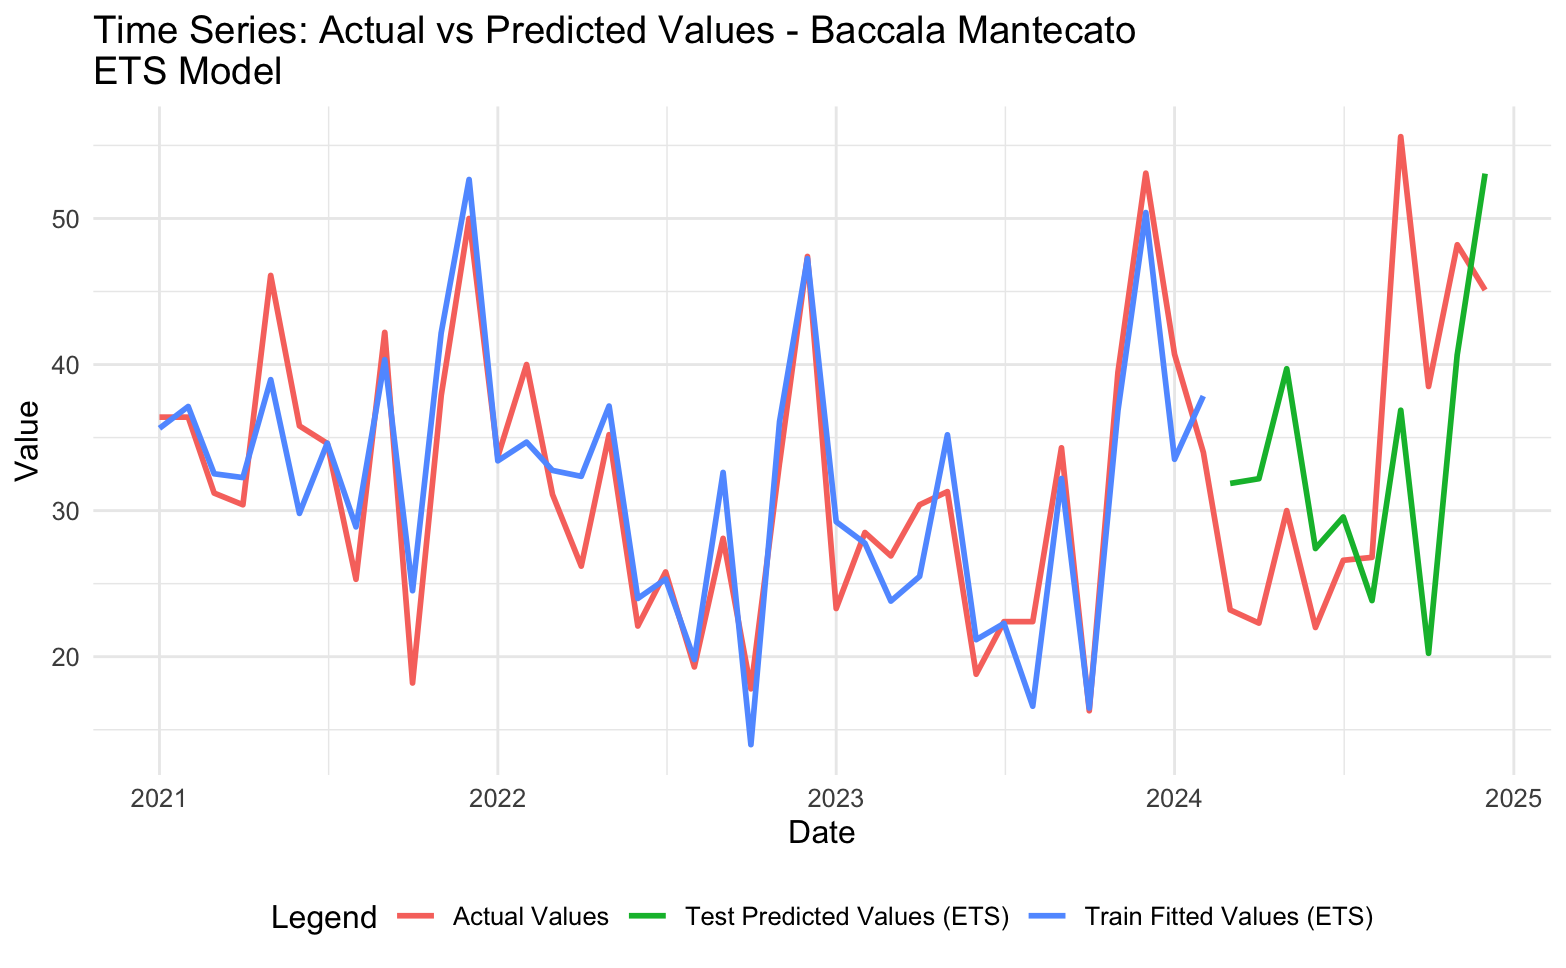
\includegraphics[width=0.5\textwidth]{PlotsBEFD/TS_M_ETS.png} 
    \caption{}
    \label{fig:esempio}
\end{figure}
The quality of the forecast was further validated by a visual comparison between the actual and predicted values. During the training phase, the forecast line closely followed the actual data, reflecting the model's ability to capture key patterns. During testing, the predictions remained near the observed values, with only minor deviations in the most extreme peaks. This consistency highlights the model's capacity to generalize and handle unseen data effectively.
We then explored more specific variants of the ETS model by introducing additive and multiplicative seasonal components through the Holt-Winters method. Using the additive approach resulted in slightly worse outcomes compared to the standard ETS model, with increases in both the Mean Squared Error (MSE) and the Akaike Information Criterion (AIC). These metrics, which are essential for evaluating model performance, indicated that the added complexity of the additive approach did not yield significant benefits. The multiplicative approach for seasonality provided even less satisfactory results, with higher errors and increased complexity, confirming that the original ETS model was the best option for this series.
\begin{table}[H]
\centering
\begin{tabular}{|l|r|r|}
\hline
\textbf{Model} & \textbf{MSE} & \textbf{AIC} \\
\hline
ETS & 111.7995 & 266.4093 \\
Holt-Winters Additive & 114.8030 & 274.4056 \\
Holt-Winters Multiplicative & 177.2098 & 274.7737 \\
\hline
\end{tabular}
\caption{Comparison of Models based on MSE and AIC | Baccalà Mantecato}
\label{table:model_comparison}
\end{table}

\subsubsection{Baccalà Vicentina}
Turning to the Baccalà Vicentina series, the behavior of the models was similar, but presented an interesting difference. Once again, the ETS model produced strong initial results, with a low MSE and a favorable AIC. However, incorporating multiplicative seasonality through Holt-Winters led to a slight reduction in MSE, albeit at the cost of a higher AIC.
\begin{table}[H]
\centering
\begin{tabular}{|l|r|r|}
\hline
\textbf{Model} & \textbf{MSE} & \textbf{AIC} \\
\hline
ETS & 1.475781 & 105.6035 \\
Holt-Winters Additive & 1.512441 & 111.4078 \\
Holt-Winters Multiplicative & 1.434768 & 109.9921 \\
\hline
\end{tabular}
\caption{Comparison of Models based on MSE and AIC | Baccalà Vicentina}
\label{table:model_comparison}
\end{table}
This trade-off between forecast accuracy and model complexity led us to select the multiplicative seasonal model as the most suitable for this series. While the increase in AIC reflected higher complexity, our primary goal of minimizing forecast errors justified this choice. By prioritizing MSE, we were able to achieve a more accurate forecast, albeit at a slightly higher computational cost.
\begin{figure}[H]
    \centering
    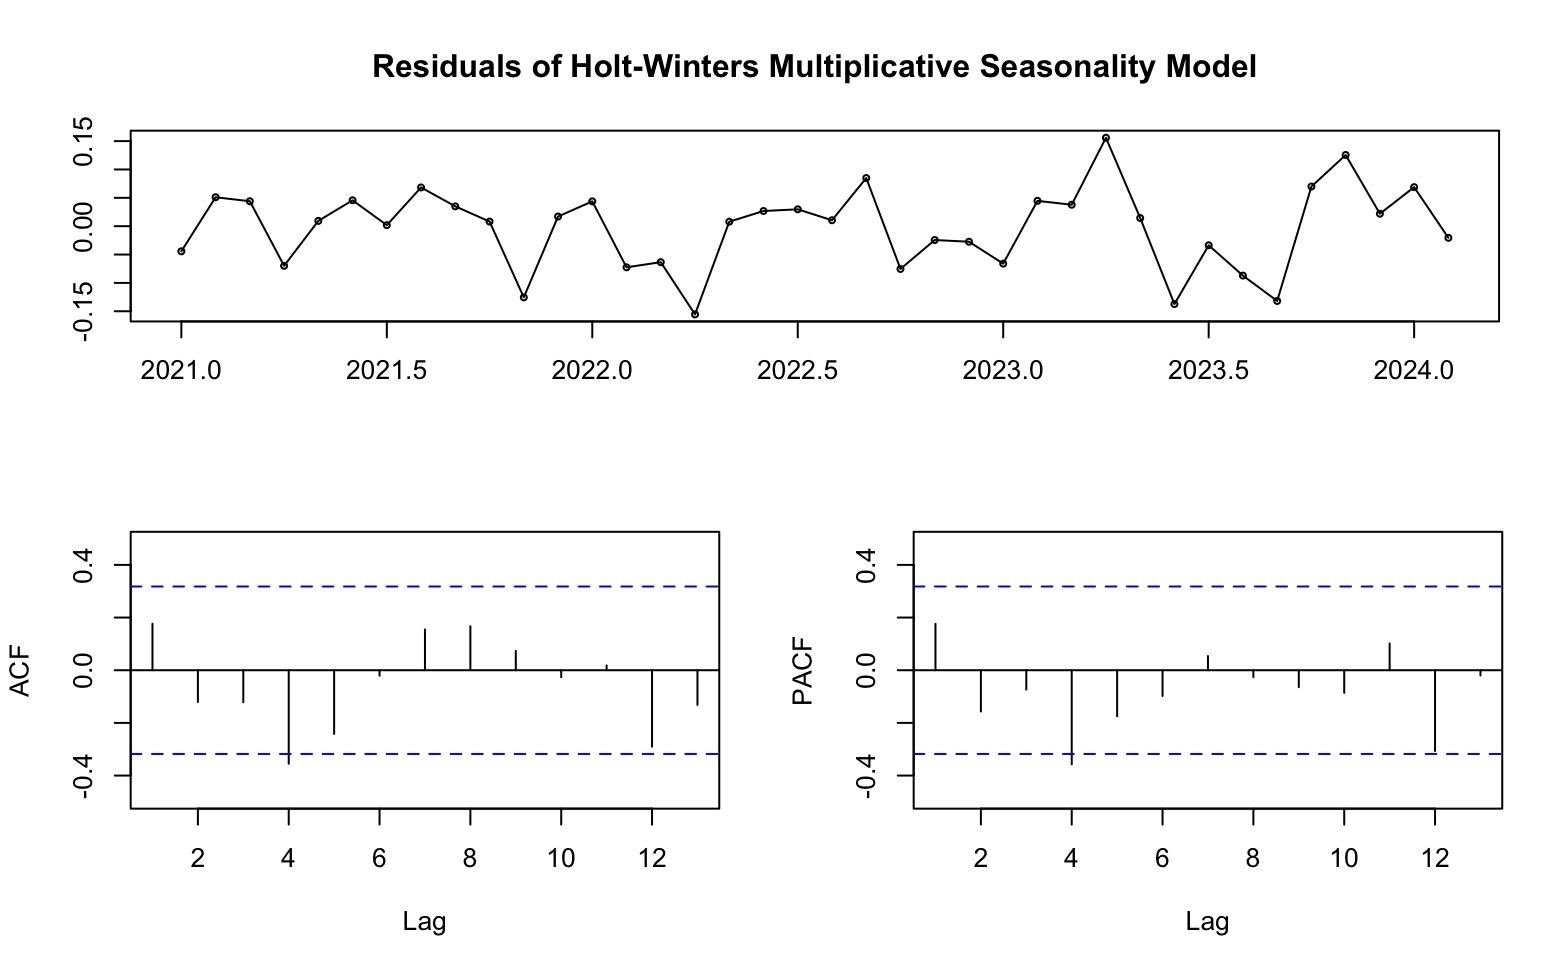
\includegraphics[width=0.5\textwidth]{PlotsBEFD/Residuals_HWM_V.png} 
    \caption{}
    \label{fig:esempio}
\end{figure}
Residual analysis confirmed that the selected models effectively captured the main characteristics of the time series. The residuals were randomly distributed around zero, showing no repeated patterns and indicating no systematic errors. The absence of significant spikes in the residuals' ACF and PACF plots further reinforced this conclusion. This is a strong indication that the chosen models are robust and reliable for forecasting purposes.
\begin{figure}[H]
    \centering
    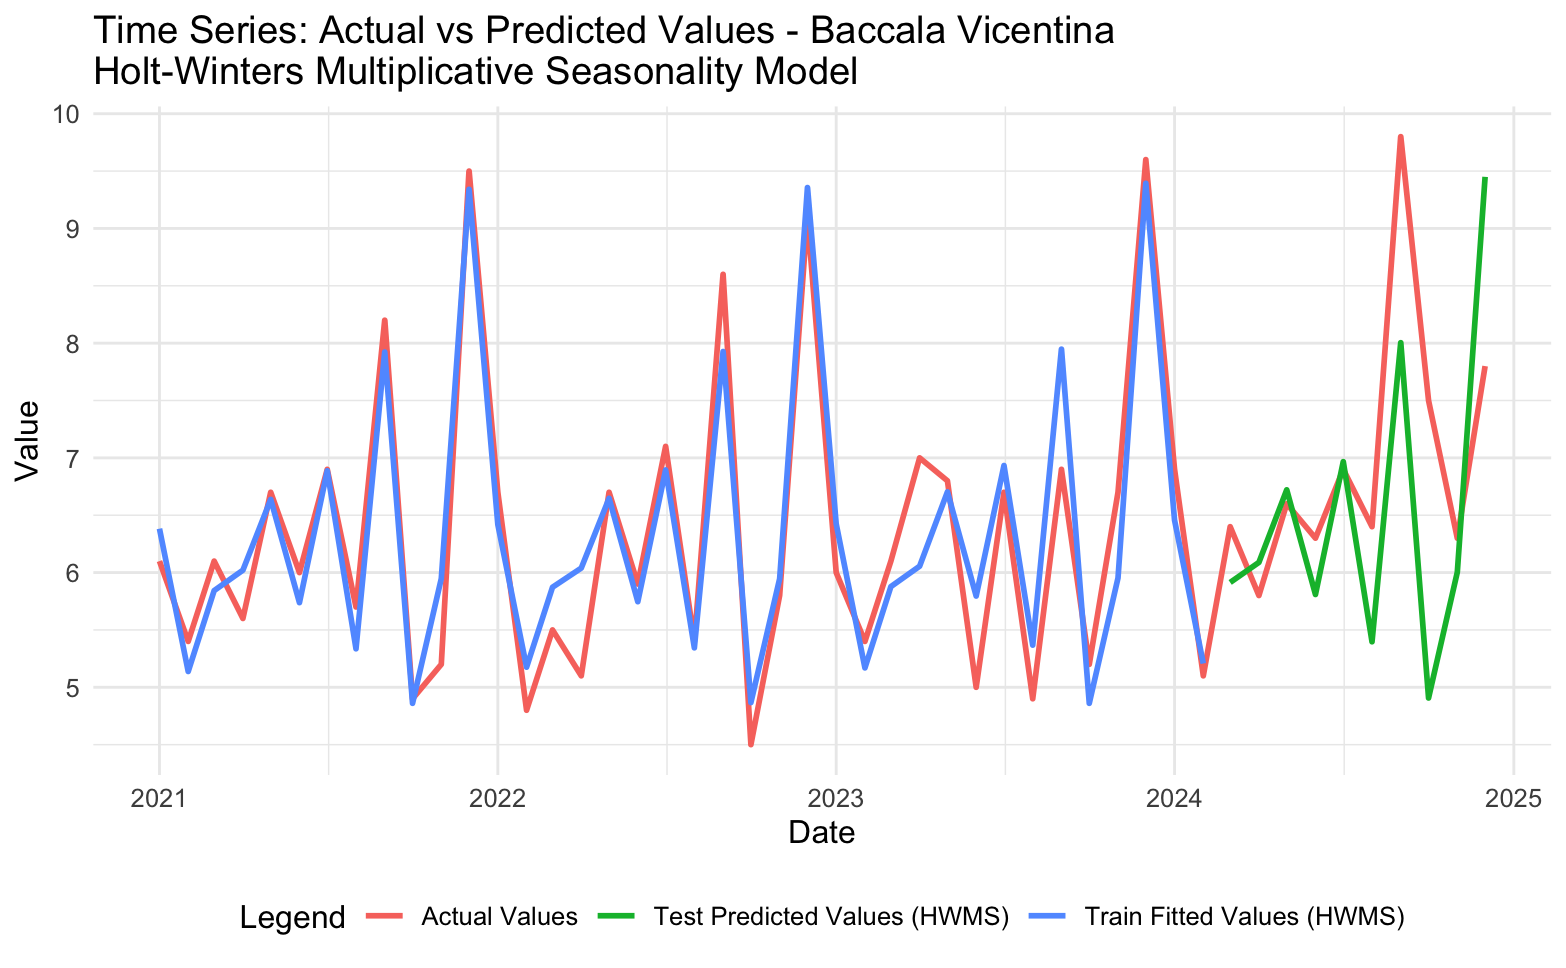
\includegraphics[width=0.5\textwidth]{PlotsBEFD/TS_HWM_V.png} 
    \caption{}
    \label{fig:esempio}
\end{figure}
Finally, the forecast plots clearly illustrated the models' ability to follow the trends and seasonality of the data in both the training and testing phases. For Baccalà Mantecato, the ETS model provided predictions that closely aligned with the actual values, though there were minor discrepancies at extreme points. For Baccalà Vicentina, the Holt-Winters model with multiplicative seasonality effectively handled the seasonal component, producing consistent forecasts. Although slight underestimations occurred at the highest peaks, overall performance remained strong.

\section{Results}

Now we compare the results of the models on the training and test sets. To do so, we create a table with the MSE values for each model on the training and test sets and plot the results.

\begin{table}[H]
\centering
\small
\begin{tabular}{|l|l|l|l|l|}
\hline
\textbf{Model} & \textbf{Train\_M} & \textbf{Train\_V} & \textbf{Test\_M} & \textbf{Test\_V} \\
\hline
\textbf{LR} & 6.7755 & 0.1879 & 45.5953 & 1.5124 \\
\textbf{SARIMA} & 29.7579 & 0.3605 & 104.5050 & 2.2650 \\
\textbf{Prophet} & 9.2290 & 0.1130 & 119.0730 & 1.8423 \\
\textbf{SARIMAX} & 14.2973 & 0.3683 & 64.0557 & 2.3494 \\
\textbf{ETS} & 13.2462 & 0.1936 & 111.7995 & 1.4348 \\
\hline
\end{tabular}
\caption{Performance metrics for different models (MSE)}
\label{table:model_comparison_inverted}
\end{table}

From the table above and subsequent plots, several insights can be drawn regarding the performance of the models.

Linear Regression is effective during training but prone to overfitting, particularly for series with complex seasonal and trend structures. While it is a simple and interpretable model, its lack of flexibility limits its applicability for forecasting. SARIMA highlights the importance of incorporating seasonality but struggles with generalization. Its poor performance during the test phase indicates that it might not be the optimal choice for these datasets. Prophet provides a balance between flexibility and complexity but falls short in test performance. Its inability to handle non-seasonal variations is a limitation in these specific contexts. SARIMAX shines as the best model for Baccalà Mantecato, showcasing the utility of external regressors. However, its mixed results for Baccalà Vicentina highlight the importance of carefully evaluating the relevance of external factors. Exponential Smoothing emerges as the best model for Baccalà Vicentina, proving its strength in handling stable seasonal series. Its consistent performance across training and test sets makes it a reliable choice.

\subsection*{Overall Insights}
For Baccalà Mantecato, SARIMAX provides the most accurate forecasts, leveraging the external regressor to enhance prediction accuracy. In contrast, for Baccalà Vicentina, Exponential Smoothing with multiplicative seasonality emerges as the top performer, balancing accuracy and simplicity. These results underscore the importance of tailoring the modeling approach to the specific characteristics of each time series.

\begin{figure}[H]
    \centering
    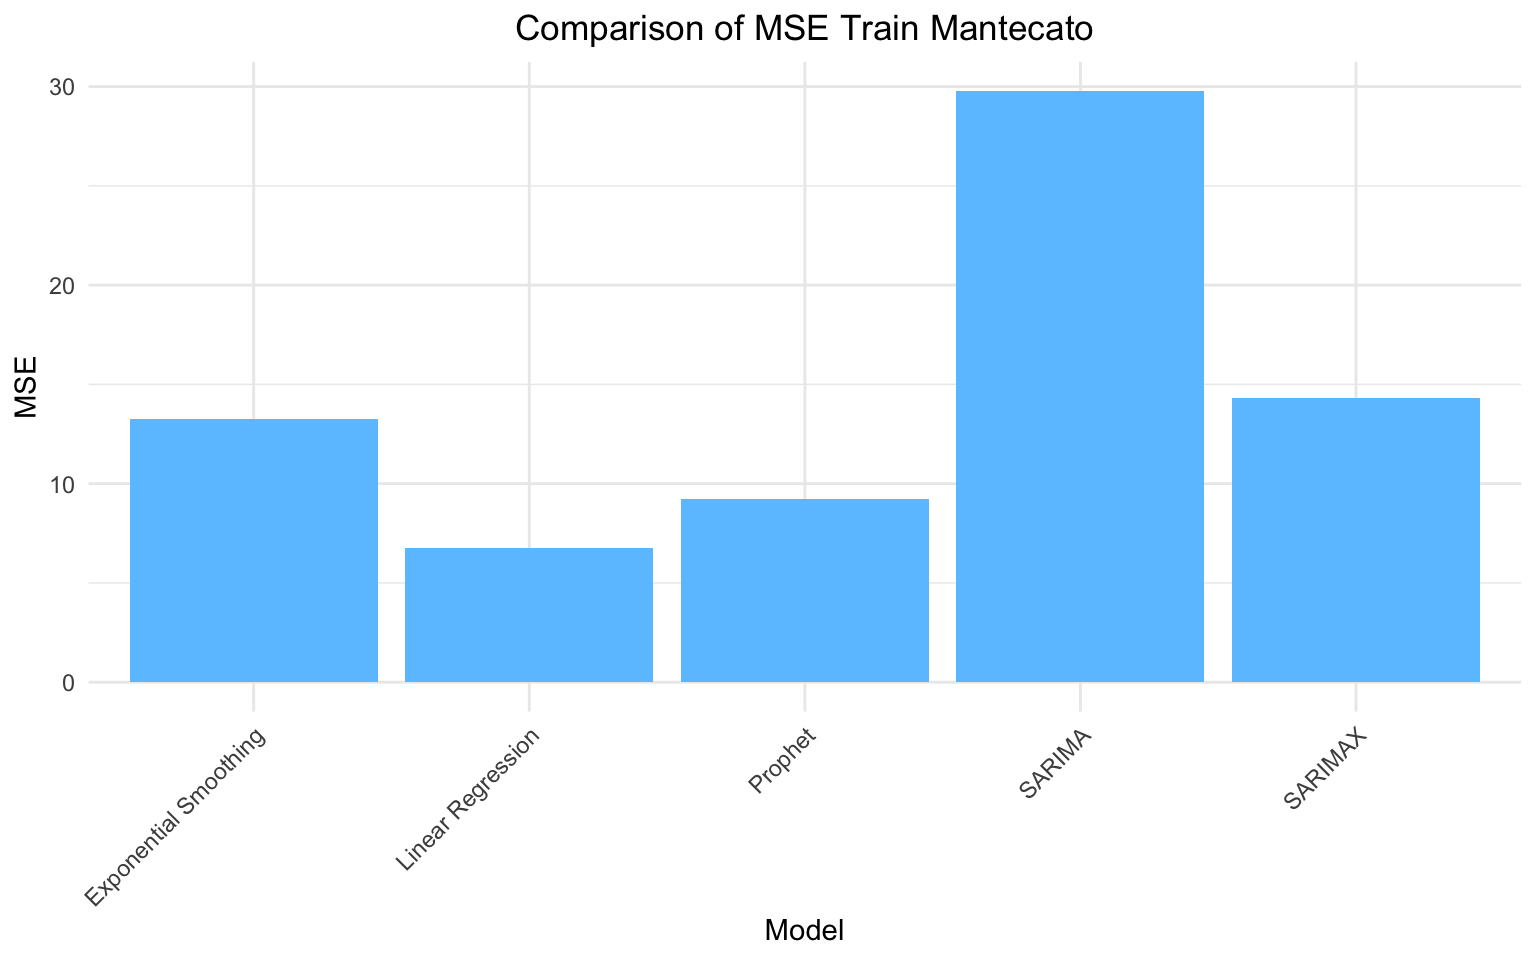
\includegraphics[width=0.5\textwidth]{PlotsBEFD/plot_results-1.png} 
    \caption{}
    \label{fig:esempio}
\end{figure}

The bar chart confirms that Linear Regression and Exponential Smoothing achieve the lowest MSE values for the training phase, indicating their ability to fit the data well. SARIMA and SARIMAX models show slightly higher training errors, which may reflect their attempt to account for more complex seasonal and trend structures.

\begin{figure}[H]
    \centering
    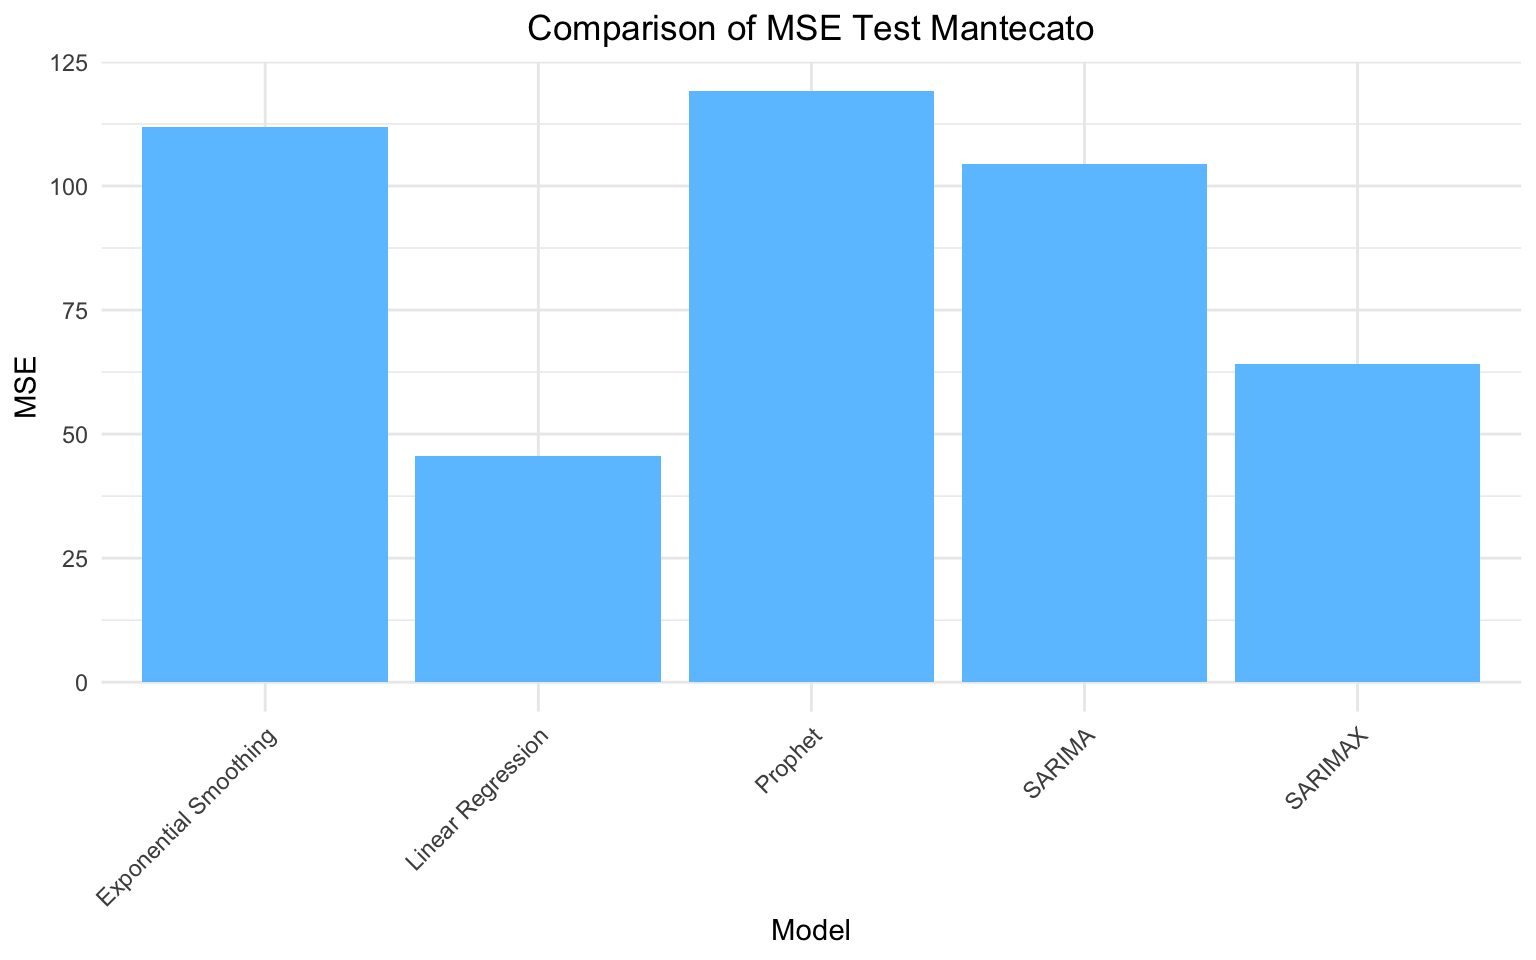
\includegraphics[width=0.5\textwidth]{PlotsBEFD/plot_results_2-1.png} 
    \caption{}
    \label{fig:esempio}
\end{figure}

The test results reveal that SARIMAX and Exponential Smoothing outperform SARIMA and Prophet models for Baccala Mantecato. The stark difference between train and test MSE for Linear Regression further highlights its overfitting issue.

\begin{figure}[H]
    \centering
    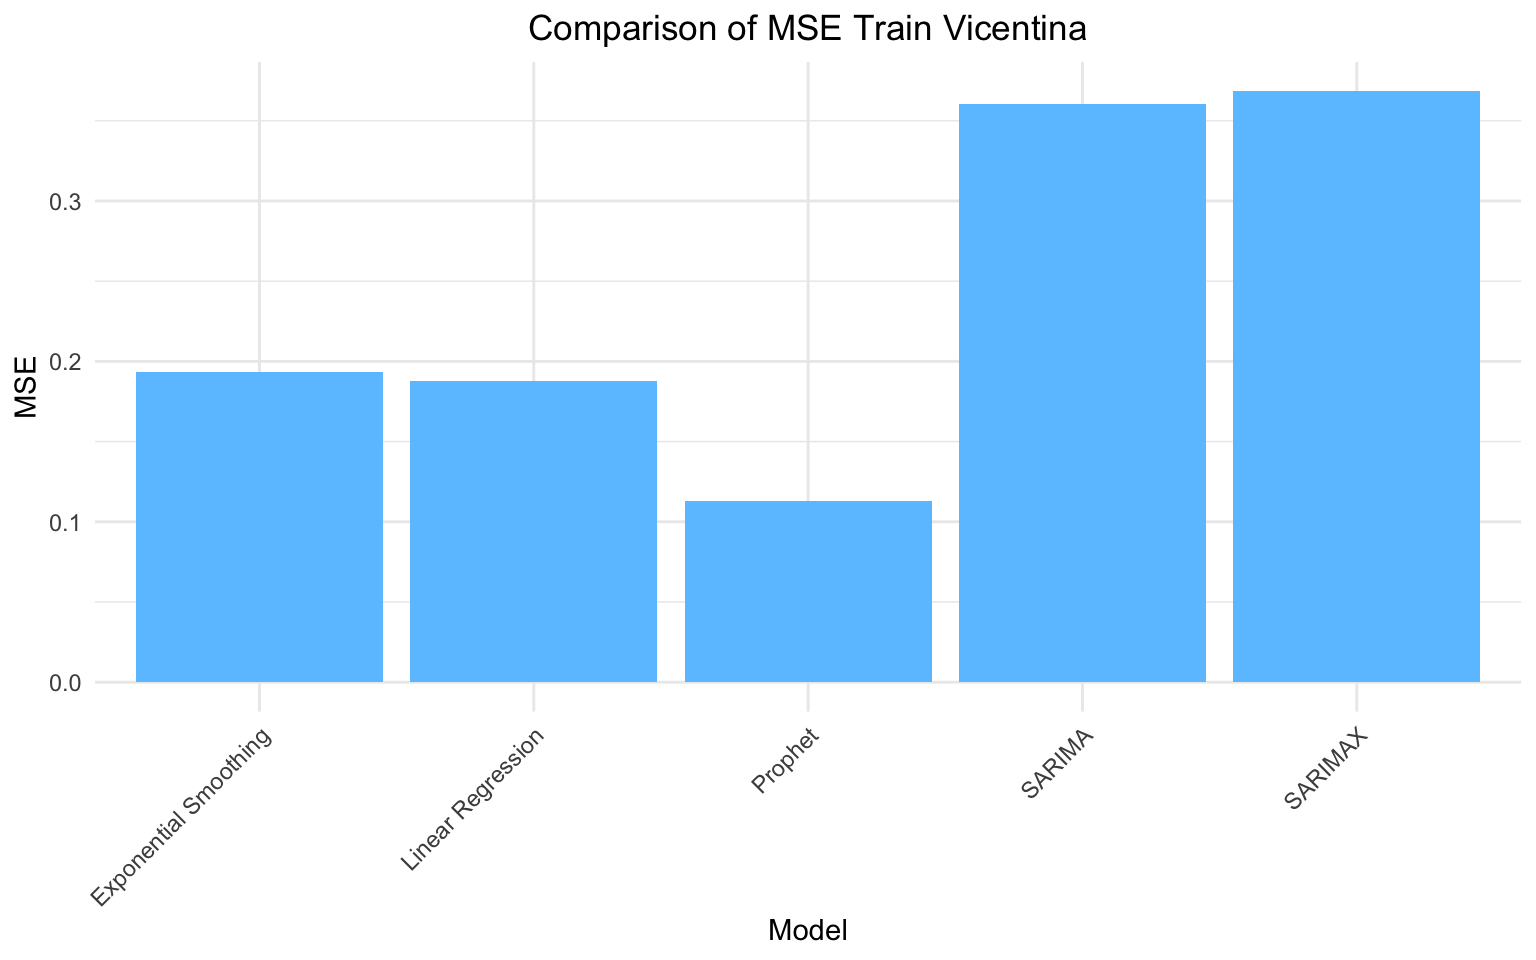
\includegraphics[width=0.5\textwidth]{PlotsBEFD/plot_results_3-1.png} 
    \caption{}
    \label{fig:esempio}
\end{figure}

Similar trends are observed for Baccala Vicentina, with Exponential Smoothing and Linear Regression performing best during training. SARIMA and SARIMAX models have noticeably higher training MSEs. The best one is the Prophet model.

\begin{figure}[H]
    \centering
    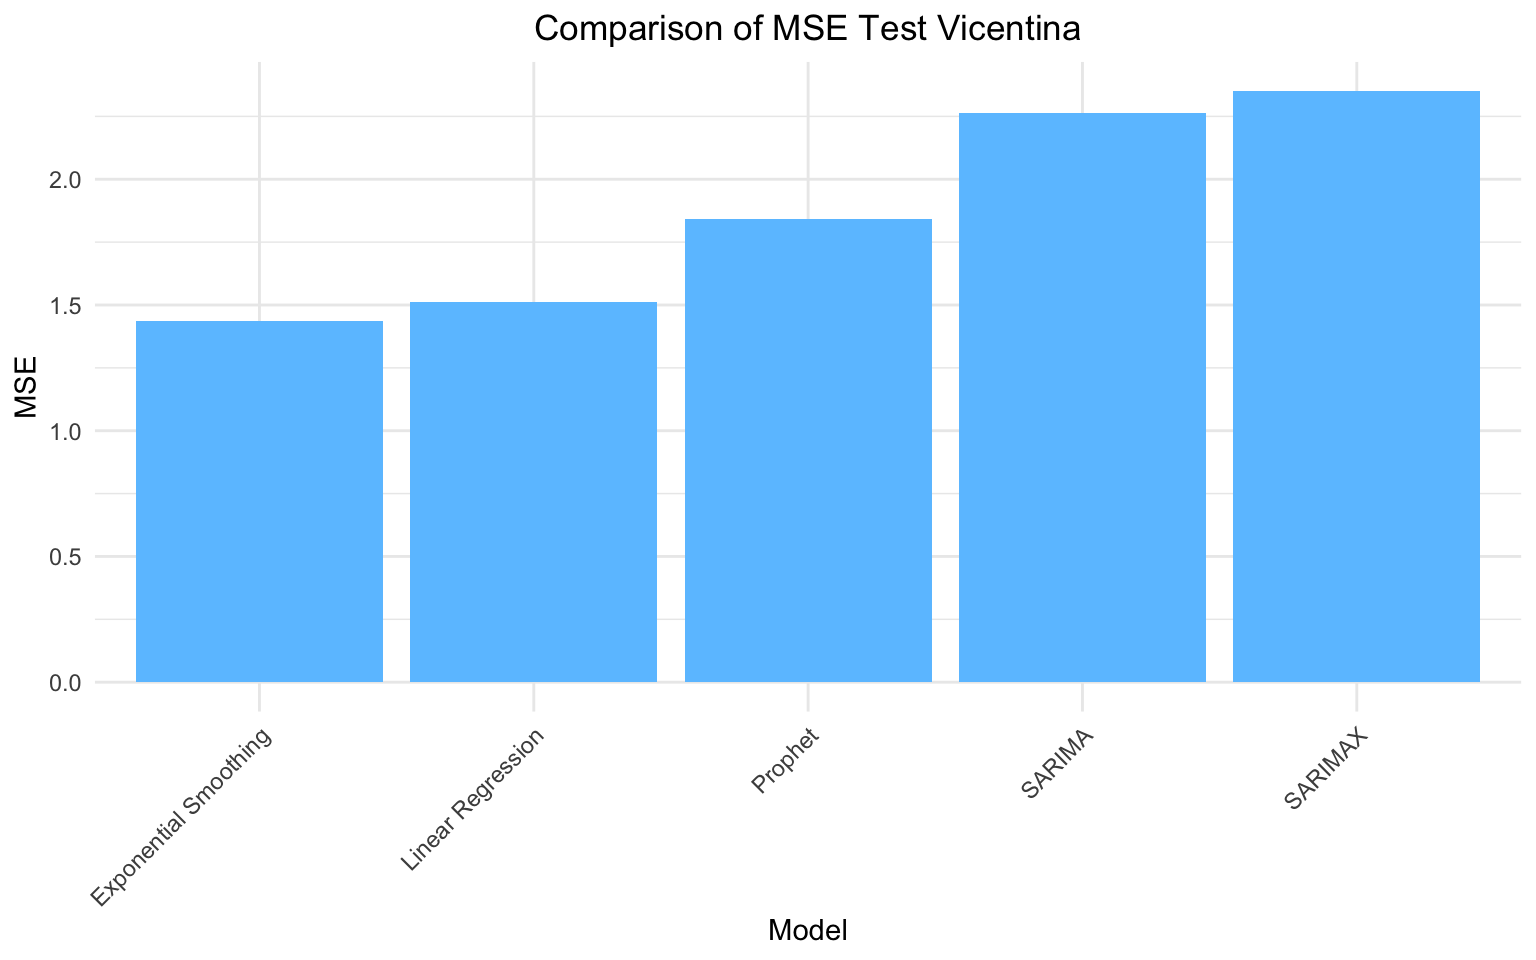
\includegraphics[width=0.5\textwidth]{PlotsBEFD/plot_results_4-1.png} 
    \caption{}
    \label{fig:esempio}
\end{figure}

For Baccala Vicentina, Exponential Smoothing slightly outperforms the other models in the test phase. SARIMA and SARIMAX perform comparably, while Prophet and Linear Regression lag behind.



\section{Conclusions}

This report demonstrates the effectiveness of various forecasting models for Baccalà Mantecato and Baccalà Vicentina, highlighting the need for tailored approaches to account for their distinct sales patterns. The findings show that no single model is optimal across both datasets, emphasizing the importance of aligning modeling techniques with the specific characteristics of the data.
For Baccalà Mantecato, SARIMAX emerged as the most effective model, leveraging external regressors such as fish consumption to significantly enhance predictive performance. This underlines the importance of integrating relevant external factors in forecasting frameworks. Conversely, for Baccalà Vicentina, Exponential Smoothing with multiplicative seasonality provided the best results, capturing the product’s stable seasonal patterns with high accuracy.
Linear Regression, while simple and interpretable, proved to be unsuitable due to overfitting and poor generalization, especially for Baccalà Mantecato. Similarly, SARIMA and Prophet, despite their capacity to model seasonal components, underperformed in the test phase, highlighting their limitations in handling complex or external dynamics.
These insights have direct implications for inventory and resource planning. The SARIMAX model for Baccalà Mantecato provides a robust framework for managing seasonal demand variability, while Exponential Smoothing ensures consistent stock levels for Baccalà Vicentina. The application of these models offers the laboratory actionable strategies to optimize production and minimize waste.

In conclusion, this analysis highlights the value of data-driven forecasting techniques to improve decision making and operational efficiency. By adopting the most suitable models for each product, the laboratory can better meet market demands while maintaining its competitive edge. Future efforts should explore integrating additional variables and advanced machine learning techniques to further refine predictive accuracy and address residual challenges.

\end{document}
